\documentclass[extra,mreferee]{gji}
%\usepackage{timet}

\usepackage{graphicx}
\graphicspath{ {./figures} }
\usepackage{subfig}
\usepackage{caption}
\usepackage{floatrow}
\usepackage{amssymb}
\usepackage{commath}
\usepackage{amsmath}

% colors to show the corrections
\usepackage[dvipsnames,usenames]{xcolor}

% colors to show the corrections
\newcommand{\red}[1]{\textbf{\textcolor{Red}{#1}}}
\newcommand{\blue}[1]{\textbf{\textcolor{Blue}{#1}}}
\newcommand{\cyan}[1]{\textbf{\textcolor{Cyan}{#1}}}
\newcommand{\green}[1]{\textbf{\textcolor{Green}{#1}}}
\newcommand{\magenta}[1]{\textbf{\textcolor{Magenta}{#1}}}
\newcommand{\orange}[1]{\textbf{\textcolor{Orange}{#1}}}

% comments between authors
\newcommand{\toall}[1]{\textbf{\orange{@@@ To all: #1 @@@}}}
\newcommand{\towenjie}[1]{\textbf{\red{*** Wenjie: #1 ***}}}
\newcommand{\tojeroen}[1]{\textbf{\green{*** Jeroen: #1 ***}}}

\floatsetup[figure]{style=plain,subcapbesideposition=top}
%\usepackage[margin=70mm]{geometry}

\title[Global Adjoint Tomography -- Model GLAD-M25]
  {Global adjoint tomography -- Model GLAD-M25\footnote{This paper is dedicated to Dimitri Komatitsch, computational geophysicist extraordinaire, who passed away unexpectedly shortly before its submission.}}

\author[Lei et al.]
  {Wenjie Lei$^1$, Youyi Ruan$^{1,2}$, Ebru Bozda\u g$^3$, Daniel Peter$^4$, Matthieu Lefebvre$^1$, \\{\LARGE \rm Dimitri Komatitsch$^5$, Jeroen Tromp$^{1,6}$, Judith Hill$^7$, Norbert Podhorszki$^7$}, \\ {\LARGE \rm and David Pugmire$^7$} \\
  $^1$ Department of Geosciences, Princeton University, Princeton, NJ 08544, USA\\
  $^2$ School of Earth Sciences and Engineering, Nanjing University, Nanjing, Jiangsu 210023, China\\
  $^3$ Department of Geophysics, Colorado School of Mines, Golden, CO 80401, USA\\
  $^4$ Extreme Computing Research Center, King Abdullah University of Science and Technology (KAUST), \\Thuwal 23955-6900, Kingdom of Saudi Arabia\\
  $^5$ LMA, CNRS UPR 7051, Aix-Marseille University, Centrale Marseille, 13453 Marseille Cedex 13, France\\
  $^6$ Program in Applied and Computational Mathematics, Princeton University, Princeton, NJ 08544, USA\\
  $^7$ Oak Ridge National Laboratory, Oak Ridge, TN 37831, USA
  }

%\newcommand{\btx}{\textsc{BibTeX}}

\begin{document}

\maketitle

%%---------------------------------------------
%
%   Summary
%
%%---------------------------------------------
\begin{summary}
Building on global adjoint tomography model~GLAD-M15~\citep{bozdaug2016global}, we present transversely isotropic global model~GLAD-M25,
which is the result of ten quasi-Newton tomographic iterations with an
earthquake database consisting of 1,480 events in the magnitude range $5.5\le M_w \le 7.2$,
an almost six-fold increase over the first-generation model.
We calculated fully 3D synthetic seismograms with a shortest period of 17~s based on a GPU-accelerated spectral-element wave
propagation solver which accommodates effects due to 3-D anelastic crust \& mantle structure, topography \& bathymetry, the ocean load, ellipticity, rotation, and self-gravitation.
We used an adjoint-state method to calculate Fr\'echet derivatives in 3D anelastic Earth models
facilitated by a parsimonious storage algorithm.
The simulations were performed on the Cray XK7 ``Titan'' and the IBM Power~9 ``Summit'' at the Oak Ridge Leadership Computing Facility.
We quantitatively evaluated GLAD-M25 by assessing misfit reductions and traveltime anomaly histograms in twelve measurement
categories.
We performed similar assessments for a held-out data set consisting of 360 earthquakes,
with results comparable to the actual inversion.
We highlight the new model for a variety of plumes and subduction zones.
\end{summary}

\begin{keywords}
Body waves, Surface waves and free oscillations, Seismic anisotropy, Seismic tomography, Computational seismology, Wave propagation, Waveform inversion
\end{keywords}

\section{Introduction}

Construction of the first seismic tomographic models of the Earth dates back to the late 1970s~\citep{Aki77,Dziewonski77,SenTok77} and early 1980s~\citep[e.g.,][]{WD84,Nataf1984}.
Around the same time,
\cite{BaChLa77}, \cite{Lailly1983}, and~\cite{Tar84} formulated and adapted the theory of adjoint-state methods~\citep{Chavent1974} for exploration seismology with the goal of capturing the full physics of seismic wave propagation.
Mainly due to computational challenges,
it took until the late 2000s to see the first applications of adjoint-state methods in regional- and continental-scale earthquake seismology~\citep{tape2009adjoint,Fichtner09,zhu2012structure}.
The first global ``adjoint tomography'' model of the Earth's mantle,
GLAD-M15, was published in 2016~\citep{bozdaug2016global}, more than 30 years after the development of the original ``full waveform inversion'' (FWI) theory.

Current global shear wavespeed models are in general agreement regardless of data type and inversion strategy in terms of long-wavelength heterogeneity \citep{ritzwollerlavely1995,TW01,beckerboschi2002}.
However, discrepancies between models become noticeable at shorter wavelengths.
Using accurate 3D simulations of seismic wave propagation and the computation of data sensitivities in 3D background models are key requirements for improving resolution in tomographic images on all scales~\citep{Tromp2020}.
Such detailed images are essential for understanding mantle dynamics and related surface tectonic processes
---for example the origin of hotspots and the driving mechanisms of plate motions and earthquakes.
Higher resolution wavespeed models are also important for accurately locating earthquakes, and are required from an engineering point of view to assess seismic hazard in earthquake prone regions and to detect and locate nuclear explosions. 

With these goals in mind,
in this study we use a GPU-accelerated version of the 3D spectral-element solver
SPECFEM3D\_GLOBE~\citep{KoTr02a,KoTr02b} on the supercomputers ``Titan'' and ``Summit'' at the Oak Ridge Leadership Computing Facility (OLCF) for global adjoint tomography.
These simulations accommodate the full 3D complexity of global Earth models,
including 3D anelastic crust and mantle structure, self-gravitation, rotation, ellipticity, topography \& bathymetry, and the load of the oceans.
No compromises are made with regards to resolving the Earth's crust,
which is explicitly captured by the spectral-element mesh~\citep{tromp2010a},
thereby eschewing the need for ubiquitous ``crustal corrections''.
The ultimate goal is to use every single piece of information in seismograms,
a task made partly feasible based on the automated window selection tool FLEXWIN~\citep{maggi2009automated}.

Global adjoint tomography has a well-defined but complex workflow with multiple stages.
% including numerical simulations of synthetic seismograms (forward simulations) for all events,
% pre-processing of seismic data, making measurements, data assimilation, Fr\'echet derivative
% calculations (adjoint simulations), and post-processing of the gradient for quasi-Newton model
% updates.
It is essential to optimize, automate, and harden the entire process using workflow management tools, especially with large data sets.
For each iteration,
1,480 forward and adjoint simulations need to be performed (one pair for each earthquake in the database),
generating a few Petabytes of wavefield files for the parsimonious-storage kernel calculation algorithm of~\cite{KoXiBoPeSaLiTr16}, and consuming 16~million OLCF node hours.

This article is organized as follows.
Section~\ref{section:seismic data} illustrates the earthquakes and seismographic stations used in the inversion,
as well as the assimilated seismic data. 
Sections~\ref{section:misfit} and~\ref{section:parameterization} describe the misfit function minimized during the inversion process
and the related model parameterization.
Section~\ref{section:misfit_evolution} describes the evolution of the misfit, and in Section~\ref{section:evaluation} we evaluate the model based on point-spread function analyses and a held-out data set of 360 earthquakes.
Finally, in Section~\ref{section:model}
we compare the results of our inversion with global shear wavespeed models 
TX2015~\citep{TX2015} and SEMUCB-WM1~\citep{french2015broad},
as well as compressional wavespeed models GAP-P4~\citep{fukao2013subducted} and UU-P07~\citep{van2018atlas}.
We conclude with a discussion of future opportunities and directions.

\section{Seismic data}
\label{section:seismic data}

Fig.~\ref{fig:eventsstations}(a) shows a map of the 1,480 earthquakes
selected from the global Centroid-Moment Tensor (CMT) catalog~\citep[e.g.,][]{ekstrom2012global}
and used in this study.
To ensure a good signal-to-noise ratio on a global scale,
the smallest moment magnitude in the database is set to~5.5,
thereby capturing more deep events,
and, to avoid complications associated with source dimension and directivity,
the largest moment magnitude is set to~7.2.
Prior to the structural inversion,
we performed source inversions using model GLAD-M15 and the CMT inversion algorithm of \cite{liu2004spectral},
as described in the Supplementary Online Material (SOM).

\begin{figure}
  \centering
  \includegraphics[width=0.8\textwidth]{figures/events_1480.pdf} \\
  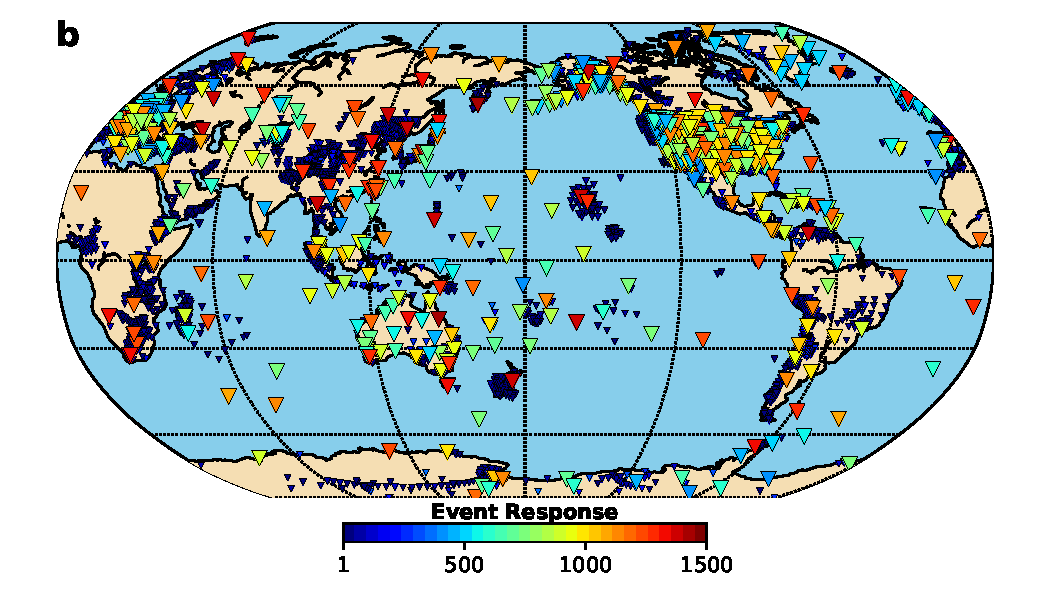
\includegraphics[width=0.8\textwidth]{figures/station_map.pdf}
  \caption{\small{(a) Distribution of 1,480~earthquakes used in this study. The color of each beach ball reflects its depth range, where blue designates events shallower than 50~km, green events between 50~km and 300~km, and red events deeper than 300~km.
  (b) Distribution of the 11,800~seismographic stations used in this study. Colors denote the number of events for which a given station contributes waveforms to the structural inversion. Stations with a number of event responses $<400$ are plotted in smaller size; these are usually temporary arrays deployed over a short period of time, frequently ocean bottom seismometers. The maximum number of event responses comes from ANMO, in Albuquerque, New Mexico, which contributed to 1,442 out of 1,480 earthquakes in the data set.
  }}
  \label{fig:eventsstations}
\end{figure}

The seismographic stations used in this study are plotted in Fig.~\ref{fig:eventsstations}(b) and
were selected to optimize global coverage
and high data quality.
In addition to the seismographic  stations used for the source inversions,
we included available data for our 1,480 event earthquake database from many data centers,
including IRIS, ORFEUS, INGV, IPGP, ETH, and GEONET.
Regional and temporary networks,
such as US Array~(TA),
Africa Array~(AF), the Canadian National Seismograph Network~(CN), Geoscience Australia~(AU),
the Antarctic Seismographic Argentinean Italian Network~(AI),
and the New Zealand National Seismograph Network~(NZ),
constitute a significant part
of our database and greatly improve coverage in certain regions.

To illustrate which seismic phases end up being assimilated,
Figs.~\ref{fig:window_density_Z}, \ref{fig:window_density_R}, and \ref{fig:window_density_T} show time-distance plots
for vertical, radial, and transverse component 17--40~s body waves,
respectively,
in which the Pyflex window count is used to identify parts of seismograms being assimilated.
The figures highlight all the well known body traveltime branches.
Collectively, the numerous compressional wave arrivals identified in Figs.~\ref{fig:window_density_Z} and~\ref{fig:window_density_R} are helpful to constrain the compressional wavespeed structure in the model.
The Pyflex window selection algorithm is currently configured not to pick body waves after the arrival of the surface waves, which is why the PcP and ScS branches are missing at shorter epicentral distances.
This is something we will reconsider in future applications by adjusting the FLEXWIN selection parameters, and perhaps also by introducing aspects of machine learning~\citep{chen2017}. 

\begin{figure}
  \centering
  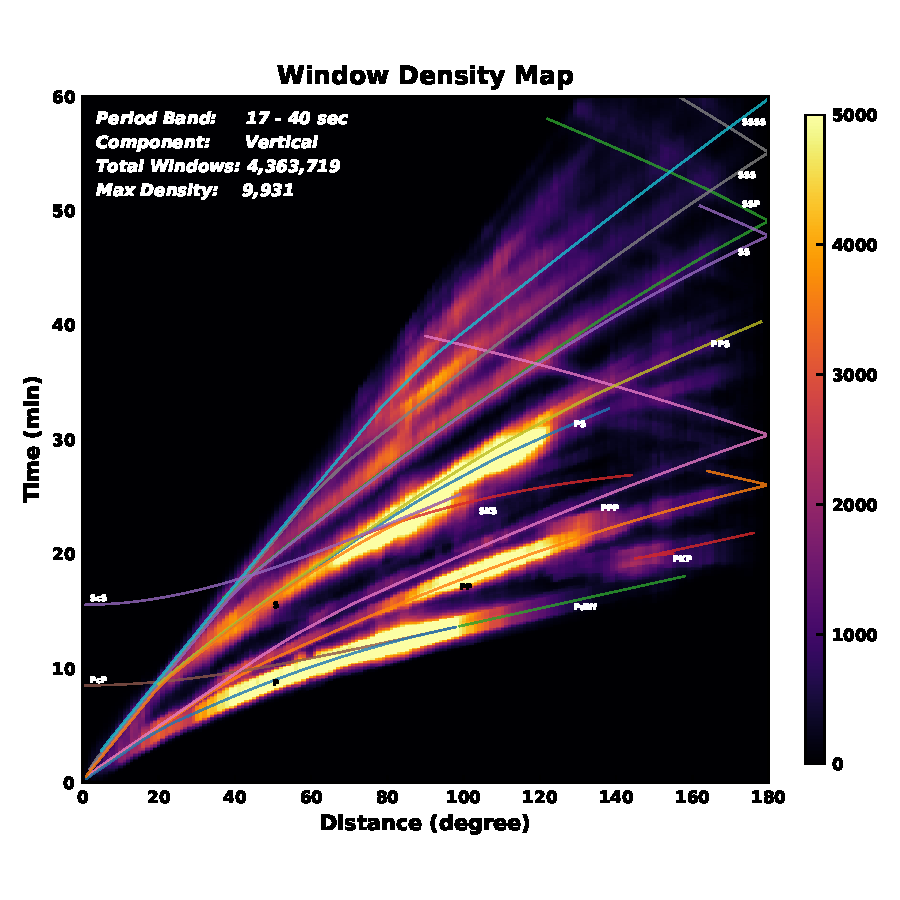
\includegraphics[width=0.9\textwidth]{figures/window_colorbar_linear_Z.pdf}
  \caption{\small{Time-distance plot for vertical component 17--40~s body waves showing a measurement window density map.
  A total of 4,363,719 time windows were discretized into 1~degree epicentral distance and 1~s time bins.
  The maximum window count is 9,931 in the 85--86$^\circ$ distance and 22~min 55~s--22~min 56~s time bin.
  Major traveltime branches are labeled. Note that the plot contains data from events with a wide variety of depths, so the branches computed for a surface focal depth are for identification purposes only.
  }}
  \label{fig:window_density_Z}
\end{figure}

\begin{figure}
  \centering
  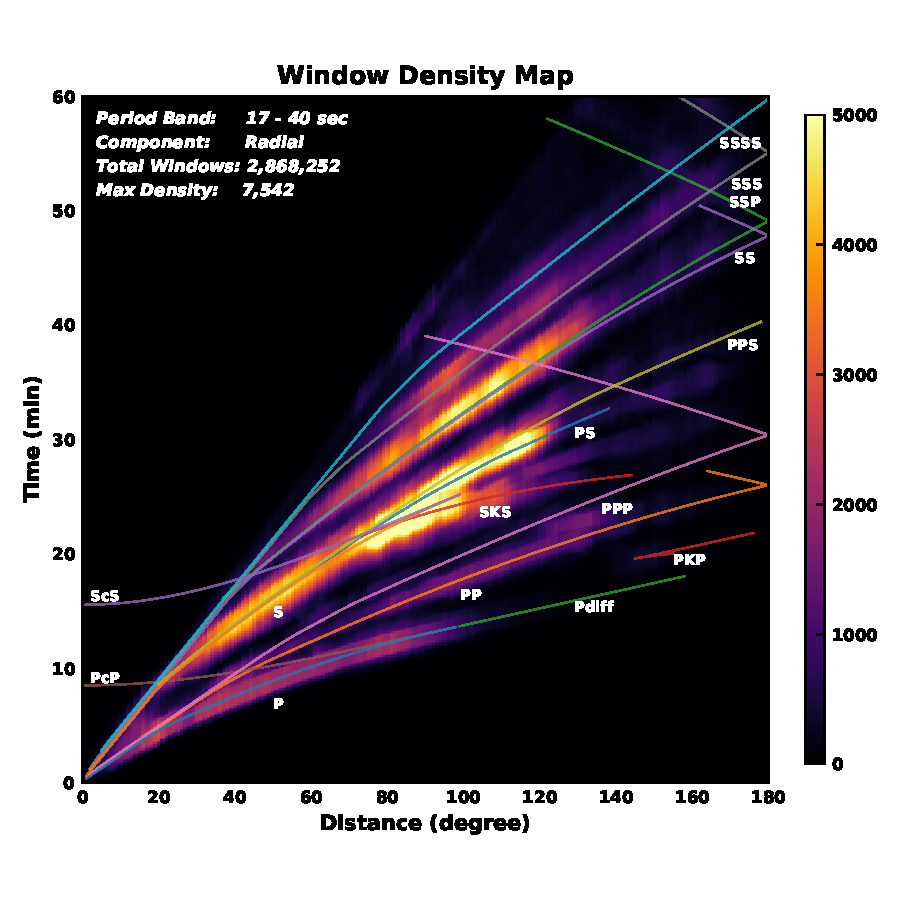
\includegraphics[width=0.9\textwidth]{figures/window_colorbar_linear_R.pdf}
  \caption{\small{Same as Fig.~\ref{fig:window_density_Z}, except for radial component 17--40~s body waves.
   A total of 2,868,252 time windows were discretized into 1~degree epicentral distance and 1~s time bins.
  The maximum window count is 7,542 in the 86--87$^\circ$ distance and 22~min 58~s--22~min 59~s time bin.
   }}
  \label{fig:window_density_R}
\end{figure}

\begin{figure}
  \centering
  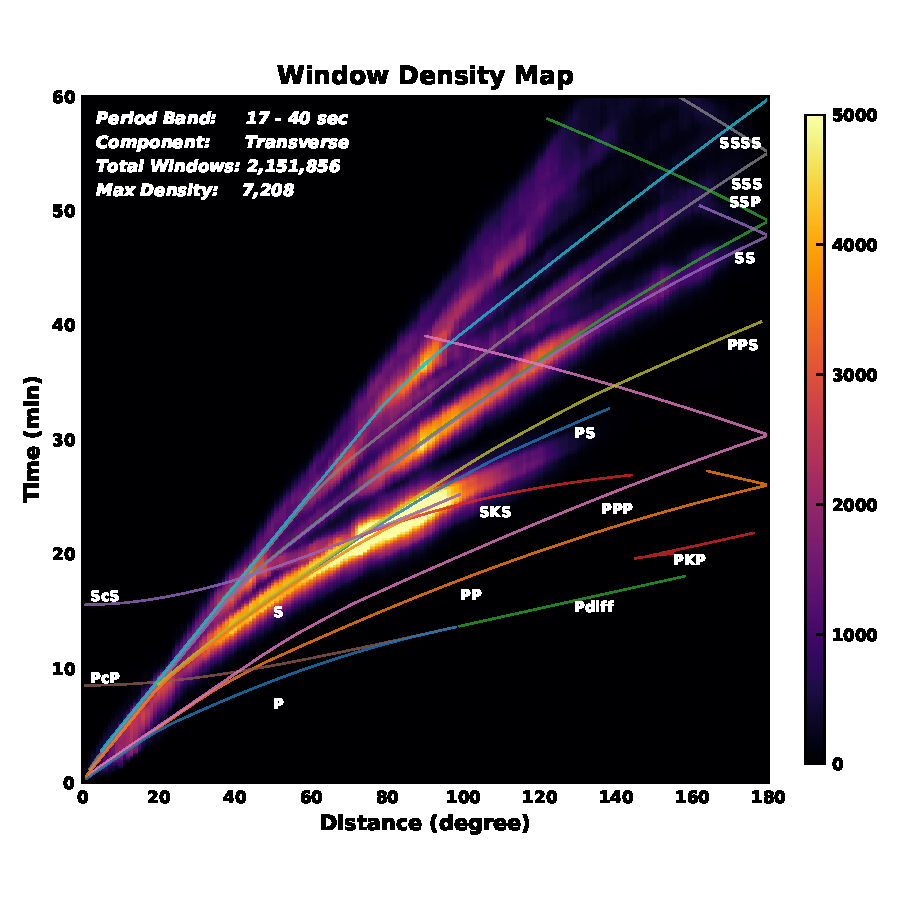
\includegraphics[width=0.9\textwidth]{figures/window_colorbar_linear_T.pdf}
  \caption{\small{Same as Fig.~\ref{fig:window_density_Z}, except for transverse component 17--40~s body waves.
   A total of 2,151,856 time windows were discretized into 1~degree epicentral distance and 1~s time bins.
   The maximum window count is 7,208 in the 89--90$^\circ$ distance and 23~min 18~s--23~min 19~s time bin.
   Only SH travetime branches are labeled.}}
  \label{fig:window_density_T}
\end{figure}

\section{Misfit function}
\label{section:misfit}

The misfit function to be minimized must
be carefully constructed.
In this study,
it involves cross-correlation traveltimes
for body waves and frequency-dependent multitaper phase measurements for surface waves.
Measurements are made in several passbands of three-component seismograms rotated
into vertical, radial, and transverse components, resulting in a number of measurement
categories.
In this study, we consider four passbands, namely, a 17--40~s passband targeting body waves,
two 40--100~s passbands separately targeting body and surface waves,
and a 90--250~s passband targeting longer-period surface waves.
Each passband involves measurements on all three components,
which results in a total of twelve measurement categories.
Although the inversion is designed to minimize the overall misfit,
we track the misfit reduction in each of the categories to ensure that
the model is improving the fit to the data roughly equally.
One of the biggest challenges in the construction of the misfit function is the
highly uneven distribution of earthquakes and seismographic stations,
which must be counterbalanced by geographically weighting the data.
This issue is discussed in detail by~\cite{Ruanetal2018};
in this section we present a brief synopsis.

With these considerations in mind,
the overall misfit, $\Phi$, is defined as follows:
\begin{equation}
\label{eq:misfit}
\Phi = \sum_{s}^{S} \omega_s \sum_{c}^{C} \omega_{c} \sum_{r}^{R_{sc}} \omega_{scr} \sum_{w}^{W_{scr}} \omega_{scrw}\, \chi_{scrw}
\quad .
\end{equation}
Here~$S$ denotes the number of sources, $C$ the number of categories,
$R_{sc}$ the number of receivers recording source~$s$ in category~$c$,
and~$W_{scr}$ the number of measurement windows for source~$s$, category~$c$,
and receiver~$r$.
The misfit for a specific source~$s$, category~$c$, receiver~$r$, and window~$w$ is
\begin{equation}
  \chi_{scrw} = \frac{1}{\Delta\omega}\int_{\omega_1}^{\omega_2} \Big( \frac {\Delta \tau_{scrw}} {\sigma_{scrw}} \Big)^2\, \mathrm{d}\omega
\quad ,
\end{equation}
where~$\Delta \tau_{scrw}$ denotes a multi-taper frequency-dependent phase measurement over the frequency interval~$\Delta\omega=\omega_2-\omega_1$\,,
with associated uncertainties~$\sigma_{scrw}$\,.
For body waves, the window misfit is often simply the cross-correlation traveltime anomaly,
$\Delta T_{scrw}$\,, weighted by its standard deviation, i.e., $\chi_{scrw}=(\Delta T_{scrw}/\sigma_{scrw})^2$\,.
The window weights are all equal, $\omega_{scrw}=1$\,,
and the category weight, $\omega_c$\,, is the reciprocal of the number of measurements in that
category, $1/C$.
Earthquakes mainly occur along plate boundaries,
and most seismographic  stations are confined to the continents,
which leads to an uneven distribution of sources and stations,
as illustrated in Fig.~\ref{fig:eventsstations}.
Therefore, weighting is crucial in global tomography to balance this uneven sampling
of Earth's interior.
Our source and receiver weighting strategy,
encapsulated by the weights~$\omega_s$ and $\omega_{scr}$\,,
is developed to compensate for uneven spatial sampling.
We define source and receiver weights as
\begin{equation}
\omega_{s}^{-1} = N\,\sum_{s'=1}^{S} \exp\left[\mbox{}-\left(\frac{\Delta_{ss'}}{\Delta}\right)^2\right]
\quad ,
\label{eq:source_weights}
\end{equation}
and
\begin{equation}
\omega_{scr}^{-1} = N_{sc}\,\sum_{r'=1}^{R_{sc}} \exp\left[\mbox{}-\left(\frac{\Delta_{rr'}}{\Delta_{sc}}\right)^2\right]
\quad ,
\label{eq:receiver_weights}
\end{equation}
respectively.
Here~$N$ and~$N_{sc}$ are normalization factors,
and~$\Delta_{ss'}$ and~$\Delta_{rr'}$ denote angular distances between source and receiver pairs~$\{s,s'\}$ and~$\{r,r'\}$\,.
The reference angular distances~$\Delta$ and~$\Delta_{sc}$ need to be chosen based on the condition 
numbers of the diagonal weighting matrices defined by Eqns.~(\ref{eq:source_weights}) and~(\ref{eq:receiver_weights}).

\section{Model parameterization}
\label{section:parameterization}

We use the same transversely isotropic model parametrization as starting model GLAD-M15.
Such a model is described by the five Love parameters $A$, $C$, $L$, $N$, and $F$~\citep{Love27},
or, alternatively, using the mass density~$\rho$, in terms of the wavespeeds~$\alpha_v=\sqrt{C/\rho}$, $\alpha_h=\sqrt{A/\rho}$, $\beta_v=\sqrt{L/\rho}$, $\beta_h=\sqrt{N/\rho}$ and the dimensionless parameter $\eta=F/(A-2L)$~\citep{PREM,DT98}.
Assuming the radial anisotropy is due to shear anisotropy, these five parameters
may be reduced to the four parameters $c$, $\beta_v$, $\beta_h$, and $\eta$ by introducing the bulk sound speed,
$c=\sqrt{\kappa/\rho}$\,.
Transverse isotropy is confined to the upper mantle; the lower mantle is assumed to be isotropic.

Since density is difficult to constrain with seismic data,
density perturbations are scaled to isotropic (Voigt averaged) shear wavespeed perturbations based on the relationship~$\delta\ln\rho = 0.33\,\delta\ln\beta$~\citep{montagner1989petrological}.

Based on this parametrization,
the variation in the misfit function~(\ref{eq:misfit}) may be expressed as~\citep{zhu2015seismic,bozdaug2016global}
\begin{equation}
    \delta \Phi = \int_V
      (\delta \ln c\,K_c + \delta \ln\beta_v\,K_{\beta_v} + \delta \ln\beta_h\,K_{\beta_h} +
      \delta\ln\eta\,K_\eta) \mathrm{d}V
      \quad ,
\end{equation}
where~$K_c$, $K_{\beta_v}$, $K_{\beta_h}$, and $K_\eta$ denote the four Fr\'echet derivatives,
which are calculated based on an adjoint-state method~\citep[e.g.,][]{Plessix_2006_RAS,Tromp2005}.


\section{Misfit evolution}
\label{section:misfit_evolution}

The inversion went through ten iterations in a number of stages, as documented
in this section. The evolution of the overall misfit function~(\ref{eq:misfit})
as well as its behavior in the various measurement categories is summarized
in Fig.~\ref{fig:misfit}.

\begin{figure}
  \centering
  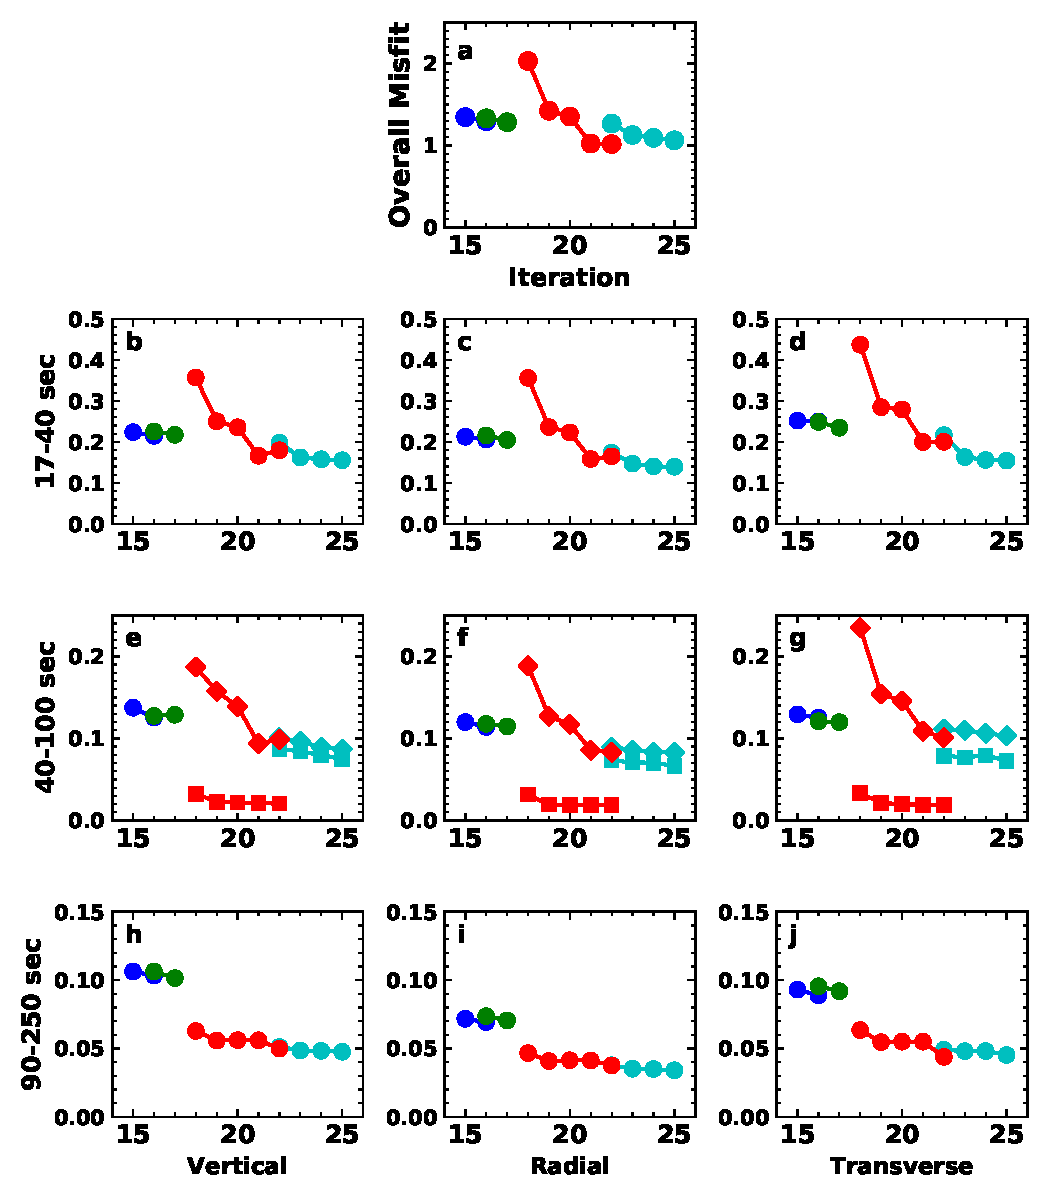
\includegraphics[width=0.8\textwidth]{figures/misfit.pdf}
  \caption{\small{Evolution of the misfit function from GLAD-M15 to GLAD-M25.
  Each color denotes different stages of the inversion, as discussed in Sections~\ref{sec:I}--\ref{sec:III}.
  (a) Evolution of the total misfit. (b)--(j) Misfit in
  each period band (rows) on three components (columns). (e)--(g) Since iteration 18,
  we  split the 40--100~s period band into two
  measurement categories: body waves (diamonds) and surface waves
  (squares).
  }}
  \label{fig:misfit}
\end{figure}

\subsection{Stage~I: Iterations 15--17}
\label{sec:I}

Starting model GLAD-M15 was constructed using a database of 253 earthquakes.
For iterations 15--17 of the inversion we used an expanded database of 520 events.
Our focus was to validate and test our software and workflow before scaling up
to a larger database of 1,040 events.
For these iterations we used three period bands, namely,
17--40~s, 40--100~s, and 90--250~s,
and we used a nonlinear conjugate
gradient method to update the model.

\subsection{Stage~II: Iterations 18--21}

The value of the misfit function changes abruptly at iteration~18
in Fig.~\ref{fig:misfit},
because of the addition of 520~events to the inversion database
and a change in the weighting strategy for 40--100~s surface waves.
For iterations 18--21 we split the 40--100~s period band into two, separating the
body and surface waves (Figs.~\ref{fig:misfit}e--g).
Since body and surface waves sample different parts of the mantle,
this split facilitated more control over the spatial distribution of the model update.
Because the 17th iteration model explains 40--100~s surface wave data relatively well,
we reduced their weight on all three components for iterations 18--21,
as indicated by the lower red curves in Figs.~\ref{fig:misfit}e--g.

The misfit reduction for 17--40~s body waves (Figs.~\ref{fig:misfit}b--d) tapers off by
iteration~21, prompting us to add more earthquakes and change the weighting strategy again by reintroducing 40--100~s surface waves.

% Table~\ref{table:measurement_category} shows the four passbands we used in Stage~II, tabulating misfit reductions in all four passbands on three components,
% that is, in twelve measurement categories.

% \begin{table}[!htb]
%   \centering
%   \begin{tabular}{|c|c|c|c|}
%     \hline
%     ~          &  Vertical & Radial &  Transverse \\
%     \hline
%     17--40~s   &   P-SV          & P-SV           & SH   \\
%     40--100~s  &   P-SV          & P-SV            & SH \\
%     40--100~s  &   Rayleigh   & Rayleigh    & Love \\
%     90--250~s  &   All                 & All                  & All  \\
%     \hline
%   \end{tabular}\\
%   \caption{\small{Twelve measurement categories used for iterations 18--25.
%   Before iteration~18, the 40--100~s body and surface waves categories were combined into a single category on each component, resulting in nine categories.}}
%   \label{table:measurement_category}
% \end{table}

\subsection{Stage~III: Iterations 22--25}
\label{sec:III}

At iteration~22 we added another 440 earthquakes to the database,
bringing the total to 1,480 events,
and we changed the 40--100~s surface wave weights back to their
setting in Stage~I. During this stage we switched from a nonlinear
conjugate gradient optimization algorithm to an L-BFGS quasi-Newton method.

\subsection{Misfit assessment}
\label{section:Misfit assessment}

In the previous sections we discussed the evolution of the misfit through
three key stages of the inversion.
``The misfit function'' is actually a different function during every iteration,
because the number of measurements continually increases as the model improves,
and the number of earthquakes increases at iterations~18 and~22.

In this section we calculate specific changes in misfit using all 1,480
earthquakes and an identical set of weights and windows for three models,
namely, GLAD-M25, GLAD-M15, and S362ANI combined with CRUST2.0.
Table~\ref{table:misfit_reduction_M15_M25} summarizes the changes in fit in
the twelve measurement categories between the new model, GLAD-M25, and its
starting model, GLAD-M15, and between GLAD-M25 and model S362ANI combined
with CRUST2.0, which was the starting model for the GLAD-M15 inversion.

We observed misfit reductions in all categories,
with dispersive 40--100~s surface waves exhibiting the largest improvements.
The improvements in fit per component are comparable in all period bands,
indicating that the various categories are reasonably well balanced in the
assessment of misfit.

\begin{table}
  \centering
  \begin{tabular}{|c|c|c|c|}
    \hline
    ~          &  Vertical (\%) & Radial (\%) &  Transverse (\%) \\
    \hline
    %17--40~s  body waves    &   17.4 (31.1)   &       21.1 (37.1) &       24.6 (42.2) \\
    %40--100~s body waves    &   16.8 (31.3)  &       21.3 (40.2)  &       21.7 (42.0) \\
    %40--100~s surface waves &   28.5 (50.1)  &       28.3 (51.1) &       28.4 (53.8)  \\
    %90--250~s surface waves &   14.5 (36.2)  &       13.4 (38.8) &       25.7 (38.6) \\
    17--40~s  body waves    &   19.1 (37.3)   &       23.7 (46.3) &       28.2 (54.8) \\
    40--100~s body waves    &   18.3 (37.5)   &       24.0 (51.4) &       24.5 (54.5) \\
    40--100~s surface waves &   33.6 (69.6)   &       33.3 (71.5) &       33.5 (77.2) \\
    90--250~s all waves &   15.7 (44.9)   &       14.4 (49.1) &       29.6 (48.7) \\
    \hline
  \end{tabular}\\
  \caption{\small{Variance reductions in the twelve measurement categories
  between the new model, GLAD-M25, and its starting model, GLAD-M15,
  and, in parentheses, between GLAD-M25 and model S362ANI combined with
  CRUST2.0, which was the starting model for the GLAD-M15 inversion.}}
  \label{table:misfit_reduction_M15_M25}
\end{table}

% \begin{table}[!htb]
%   \centering
%   \begin{tabular}{|c|c|c|c|}
%     \hline
%      ~          &  Vertical(\%) & Radial(\%) &  Transverse(\%) \\
%     \hline
%     17--40s body waves     &    31.1    &       37.1 &       42.2 \\
%     40--100s body waves    &    31.3    &       40.2 &       42.0 \\
%     40--100s surface waves &    50.1    &       51.1 &       53.8 \\
%     90--250s               &    36.2    &       38.8 &       38.6 \\
%     \hline
%   \end{tabular}\\
%   \caption{\small{Misfit Reduction from M00 to M25 for 1480 earthquakes used in the inversion.}}
%   \label{table:misfit_reduction_M00_M25}
% \end{table}

\subsection{Histogram comparisons}
\label{section:Histogram comparisons}

Another way to evaluate model quality is by assessing the distribution
of measurements in the various categories.
Again we use all 1,480 events and a set of identical windows on all three components
to assess GLAD-M25, GLAD-M15, and S362ANI combined with CRUST2.0.
The total number of selected windows,
determined using model GLAD-M25, exceeds 18~million.
Fig.~\ref{fig:phase_hist} shows histograms of the resulting phase
measurements in all twelve measurement categories.
We observe that the distributions generally become better centered on zero,
and that all standard deviations are steadily reduced.
The inversion is aimed at reducing the overall misfit,
so there are small tradeoffs between different measurement categories.

\begin{figure}
  \centering
  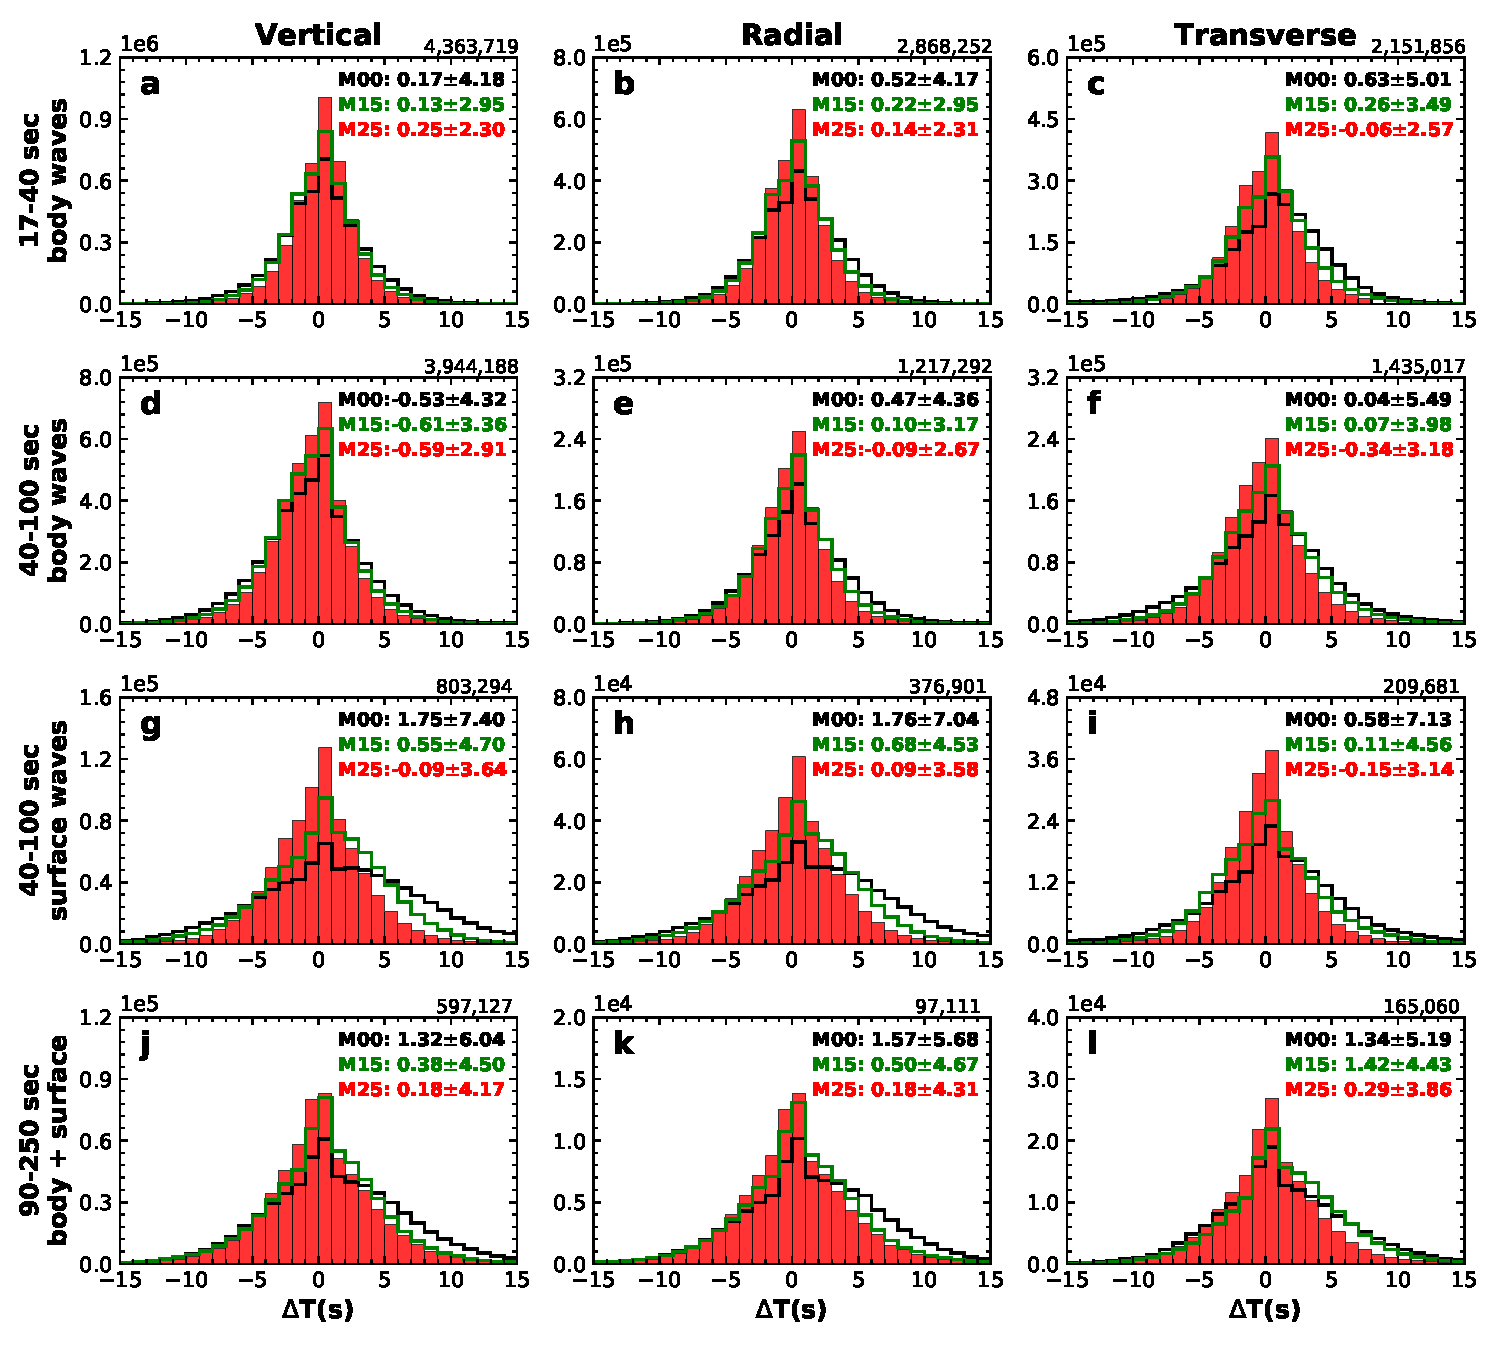
\includegraphics[width=\textwidth]{figures/dt_histogram.pdf}
  \caption{\small{Histograms of phase measurements in all twelve measurement categories for S362ANI combined with CRUST2.0 (M00, Black), GLAD-M15 (M15, Green), and GLAD-M25 (M25, Red).
  Each column represents one component and each row corresponds to a period band.
  The numbers above the top right of each panel denote the number of measurements in the corresponding category.
  The total number of measurements is 18.2~million.
  The mean and standard deviations of the phase measurements for the three models are displayed in the top right corner of each panel.}}
  \label{fig:phase_hist}
\end{figure}

\section{Model evaluation}
\label{section:evaluation}

% In this section we evaluate model GLAD-M25 further based on a point-spread
% function resolution analysis as well as a ``held-out'' data set, that is,
% a set of data not used in the actual structural inversion.

\subsection{Point-spread function analyses}

Checker-board tests or tests involving a chosen known structure, e.g., a plume or slab,
are frequently used to assess the quality of a tomographic inversion,
despite the fact that such tests have limited relevance~\citep[e.g.,][]{Leveque1993}.
Such tests are computationally expensive in FWI and adjoint tomography, because they
require roughly the same computational resources as the actual inversion.
In lieu of such tests, we previously performed two point-spread function (PSF) analyses~\citep{fichtner2011resolution}
for model GLAD-M15~\citep{bozdaug2016global}.
Here we repeat one of those tests (underneath Yellowstone) to show the improved resolution in GLAD-M25 relative to GLAD-M15,
and we perform three additional PSF tests: in the lower mantle underneath Afar, in the lower mantle beneath Easter Island, and below the transition zone in Sumatra.
Two additional PSF tests for anomalies below the US may be found in the SOM.

A PSF test is based on the relationship
\begin{equation}
    \mathsf{H}\cdot\mathsf{\Delta}\mathsf{m}\approx\mathsf{g}(\mathsf{m}+\mathsf{\Delta}\mathsf{m})-\mathsf{g}(\mathsf{m})
    \quad .
\end{equation}
This expression states that the action of the Hessian~$\mathsf{H}$ on a model perturbation~$\mathsf{\Delta}\mathsf{m}$ maybe calculated by taking the difference between the misfit gradient at model~$\mathsf{m}+\mathsf{\Delta}\mathsf{m}$ and the misfit gradient at model~$\mathsf{m}$\,.
Thus, such a test has a computational cost that is equivalent to one iteration, because it only requires the calculation of the gradient~$\mathsf{g}(\mathsf{m}+\mathsf{\Delta}\mathsf{m})$\,.
At a minimum of the misfit function,
perturbations in displacement~$\Delta\mathbf{s}$ are proportional to model parameter perturbations~$\mathsf{\Delta}\mathsf{m}$\,, that is~$\Delta\mathbf{s}\sim\mathsf{\Delta}\mathsf{m}$\,.
Consequently, if we perturb model parameter~$k$ at location~$\mathbf{x}$\,,
$\Delta m_k(\mathbf{x})$\,,
we expect that the only nonzero element of the Hessian matrix is~$H_{kk}(\mathbf{x})$, and that~$\mathsf{H}\cdot\mathsf{\Delta}\mathsf{m}\sim\Delta m_k(\mathbf{x})$\,.
Thus a PSF test illustrates the degree of blurring or smearing of the induced model perturbation~$\Delta m_k(\mathbf{x})$ and identifies tradeoffs with other model parameters.

Fig.~\ref{fig:psf_tests} shows the results of the four PSF tests we performed for model GLAD-M25.
The first test repeats an analysis performed by~\cite{bozdaug2016global} for GLAD-M15 in the upper mantle underneath Yellowstone.
That test was based on 253 earthquakes,
and Figs.~\ref{fig:psf_tests}a shows our result for the same location based on the current dataset of 1,480 events.
We observe that the 100~km diameter anomaly at 300~km depth is well recovered, with little tradeoff between~$\beta_\mathrm{V}$ and~$\beta_\mathrm{H}$ and~$c$ (See SOM).
Figs.~\ref{fig:psf_tests}b--d shows the results of PSF tests in the lower mantle beneath Afar,
in the lowermost mantle beneath Easter Island,
and in the mid mantle below Sumatra.
In each case the Gaussian anomaly is well recovered, with minimal tradeoff with other model parameters (See SOM).

\begin{figure}
  \centering
  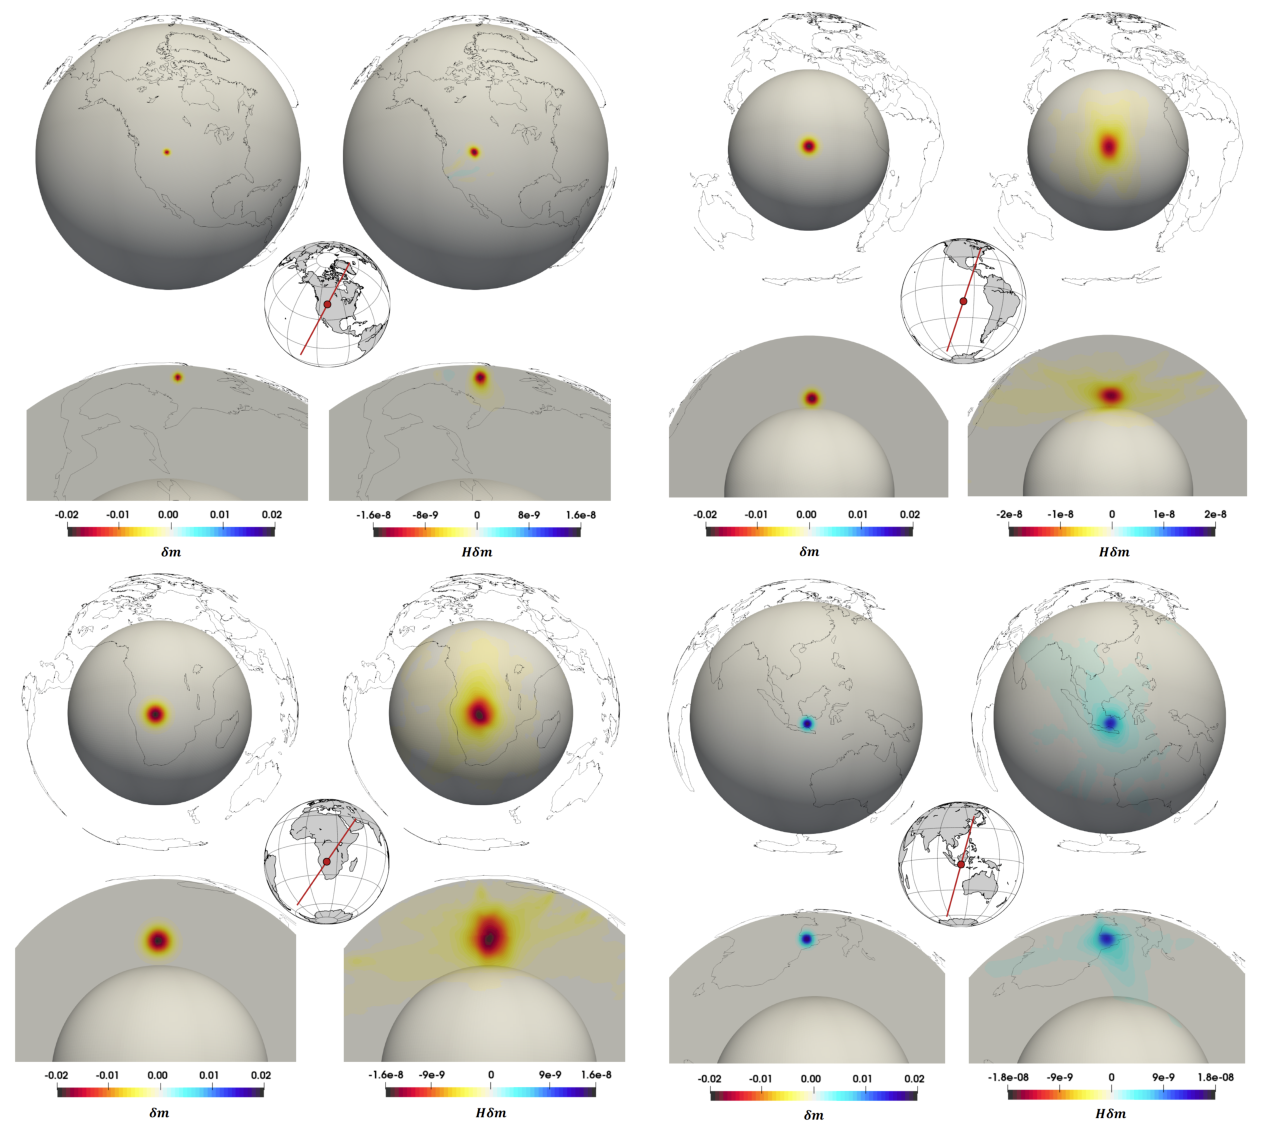
\includegraphics[width=\textwidth]{figures/psf/psf_tests.pdf}
  \caption{\small{PSF tests.
  Each of the four panels labeled (a)--(d) shows a map view (Top Left) and cross section (Top Right) through a Gaussian perturbation, $\mathsf{\Delta}\mathsf{m}$\,, in~$\beta_\mathrm{V}$\,,
  and a map view (Bottom Left) and cross section (Bottom Right) through the recovered perturbation, $\mathsf{H}\cdot\mathsf{\Delta}\mathsf{m}$\,, in~$\beta_\mathrm{V}$.
  (a) 100~km diameter negative Gaussian anomaly at a depth of 300~km beneath Yellowstone.
  (b) 400~km diameter negative Gaussian anomaly at a depth of 2,000~km beneath Afar.
  (c) 300~km diameter negative Gaussian anomaly at a depth of 2,500~km beneath Easter Island.
  (d) 200~km diameter positive Gaussian anomaly at a depth of 900~km beneath Sumatra.
  }}
  \label{fig:psf_tests}
\end{figure}

\subsection{Held-out data set}

\begin{figure}
  \centering
  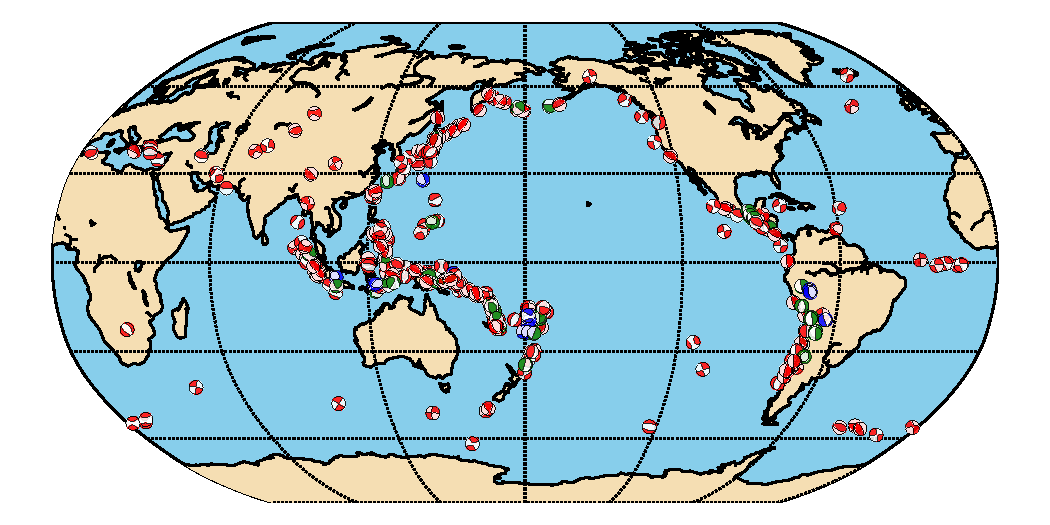
\includegraphics[width=0.8\textwidth]{figures/events_360.pdf}
  \caption{\small{Held-out database containing 360 earthquakes. These events were not used in the structural inversion and are color coded by depth range as in Fig.~\ref{fig:eventsstations}(a).}}
  \label{fig:events_360}
\end{figure}

Following the approach of \cite{tape2009adjoint}, \cite{chen2015multiparameter},
and \cite{bozdaug2016global}, we selected 360 earthquakes that were not used
in the actual inversion. This held-out data set consists of all magnitude 6.3--7.0
earthquakes in the global CMT catalog that were not used in the inversion.
We chose larger events to generate as many measurements as possible.
We calibrated the centroid time and scalar moment using a grid search based on
3D synthetics calculated in GLAD-M25.
Fig.~\ref{fig:events_360} summarizes the properties of the held-out database.

First, we repeated the misfit assessment discussed in
Section~\ref{section:Misfit assessment} for the held-out database.
Table~\ref{table:misfit_reduction_M15_M25_360} summarizes the reductions
in misfit for the held-out database for model GLAD-M25 compared to GLAD-M15
as well a S362ANI combined with CRUST2.0.
It is encouraging to see that the reductions are comparable to the
values tabulated in Table~\ref{table:misfit_reduction_M15_M25} for the actual inversion.
Overall, the reductions are slightly smaller, partly due to the fact that we did not
conduct full CMT inversions for the held-out database.

\begin{table}
  \centering
  %\label{tab:category}
  \begin{tabular}{|c|c|c|c|}
  \hline
  ~          &  Vertical (\%) & Radial (\%) &  Transverse (\%) \\
  \hline
  17--40~s                &          11.8 (29.2) &       14.1 (33.7) &       21.5 (43.4) \\
  40--100~s body waves    &          14.5 (26.2) &       12.9 (32.2)  &       16.9 (39.0) \\
  40--100~s surface waves &          29.3 (49.1) &       28.1 (49.4) &       23.7 (51.2) \\
  90--250~s               &          10.9 (30.9) &       14.3 (34.8)  &       24.0 (34.9) \\
  \hline
  \end{tabular}\\
  \caption{\small{Changes in fit for 360 earthquakes not used in the inversion in the twelve measurement categories
between the new model, GLAD-M25, and its starting model, GLAD-M15, and, in parentheses, between GLAD-M25 and model S362ANI combined with CRUST2.0, which was the starting model for the GLAD-M15 inversion.}}
  \label{table:misfit_reduction_M15_M25_360}
\end{table}

% \begin{table}[!htb]
%   \centering
%   %\label{tag:misfit_reduction_M00_M25_360}
%   \begin{tabular}{|c|c|c|c|}
%     \hline
%     ~          &  Vertical(\%) & Radial(\%) &  Transverse(\%) \\
%     \hline
%     17--40s                &         29.2 &       33.7 &       43.4 \\
%     40--100s body waves    &         26.2 &       32.2 &       39.0 \\
%     40--100s surface waves &         49.1 &       49.4 &       51.2 \\
%     90--250s               &         30.9 &       34.8 &       34.9 \\
%     \hline
%   \end{tabular}\\
%   \caption{\small{Misfit Reduction from M00 to M25 for 360 earthquakes as held-out data set.}}
%   \label{table:misfit_reduction_M00_M25_360}
% \end{table}

\begin{figure}
  \centering
  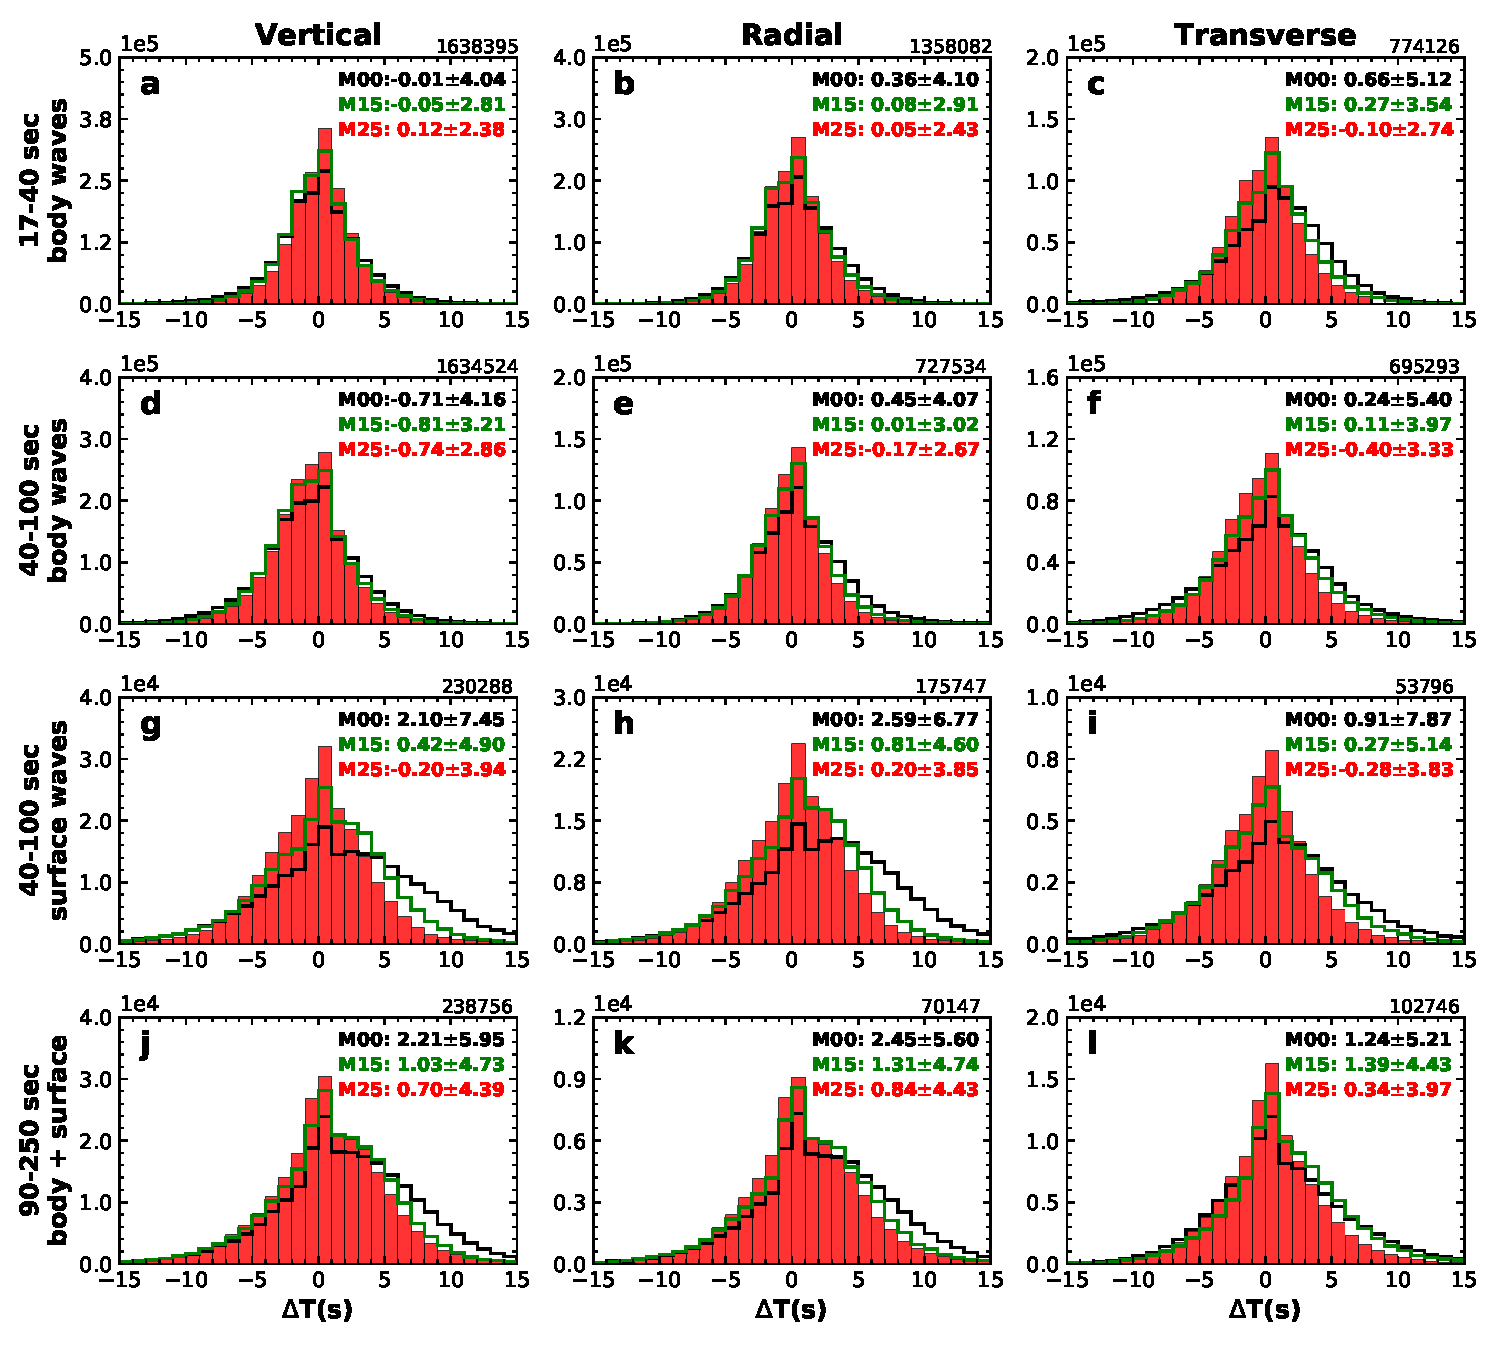
\includegraphics[width=\textwidth]{figures/dt_histogram_360.pdf}
  \caption{\small{Same as Fig.~\ref{fig:phase_hist}, except for the held-out database.
  }}
  \label{fig:phase_hist_360}
\end{figure}

% \begin{figure}
%   \centering
%   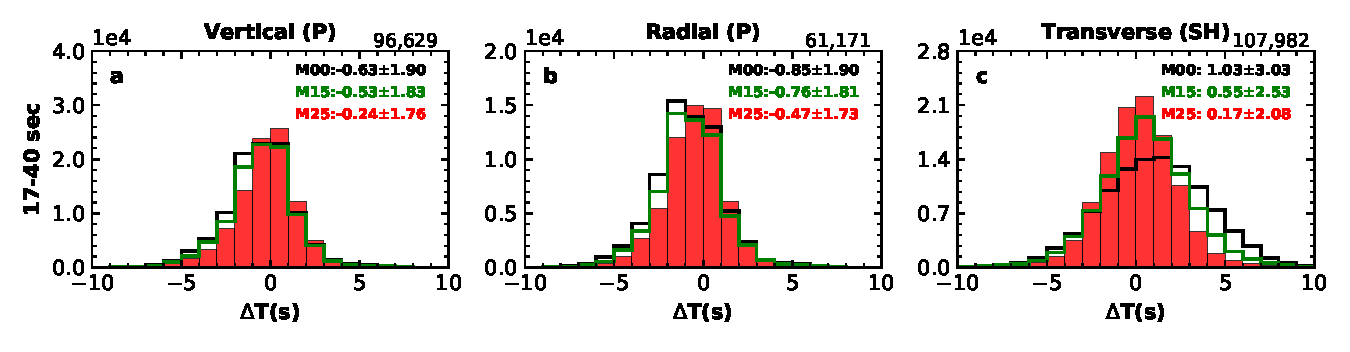
\includegraphics[width=\textwidth]{figures/dt_histogram_360_phase.pdf}
%   \caption{\small{Same as Fig.~\ref{fig:PS_phase_hist}, except for the held-out database.}}
%   \label{fig:phase_hist_360_P}
% \end{figure}

Second, we repeated the histogram comparisons discussed in
Section~\ref{section:Histogram comparisons} for the held-out database.
We used a set of identical windows on all three components to assess
phase anomalies in models GLAD-M25, GLAD-M15, and S362ANI combined with CRUST2.0.
Fig.~\ref{fig:phase_hist_360} shows histograms of the resulting phase
measurements in all twelve measurement categories.
The total number of measurements exceeds 7.8~million.
As in the actual inversion,
we observe systematic decreases in all standard deviations in all twelve categories,
and we note a sharpening of the distributions centered around zero.

% Finally,
% direct P and S traveltime anomaly measurements were extracted and compared for three models in Fig.~\ref{fig:phase_hist_360_P}.
% Again the histograms are consistent with the actual inversion,
% as expected.

\section{Model GLAD-M25}
\label{section:model}

In this section we compare model GLAD-M25 with GLAD-M15,
global shear wavespeed models 
TX2015~\citep{TX2015} and SEMUCB-WM1~\citep{french2015broad},
and compressional wavespeed models GAP-P4~\citep{fukao2013subducted} and UU-P07~\citep{van2018atlas}.
The focus is on isotropic shear and compressional wavespeed variations.
We refrain from detailed tectonic/geodynamic interpretations,
which will be the subject of more targeted future investigations.
Our goal in the article is to discuss the construction of model GLAD-M25,
and to place it into a broader tomographic context. 

Vertical cross sections are plotted relative to the spherical average of GLAD-M25,
as discussed in Appendix~\ref{sec:1Dmodel}.
For plotting purposes and use in other applications,
an expansion of the model in spherical harmonics and radial B-splines is
discussed in Appendix~\ref{sec:shanalysis}.

\subsection{Comparisons with GLAD-M15}

Relative to our first generation model GLAD-M15,
we observe a significant increase in model perturbation amplitudes and resolution,
both in the upper and lower mantle.
To illustrate this point,
Fig.~\ref{fig:power} and Fig.~\ref{fig:powerspectraradius} show normalized power per angular degree (Eqn.~\ref{eq:powerdegree}) and normalized power per angular degree as a function of radius (Eqn.~\ref{eq:powerdegreeradius}), respectively, for models S362ANI, GLAD-M15, and GLAD-M25.
Model S362ANI has no power beyond degree~18,
and we see and increase in power for GLAD-M25 relative to GLAD-M15 beyond degree~10 throughout the mantle.

\begin{figure}
  \centering
  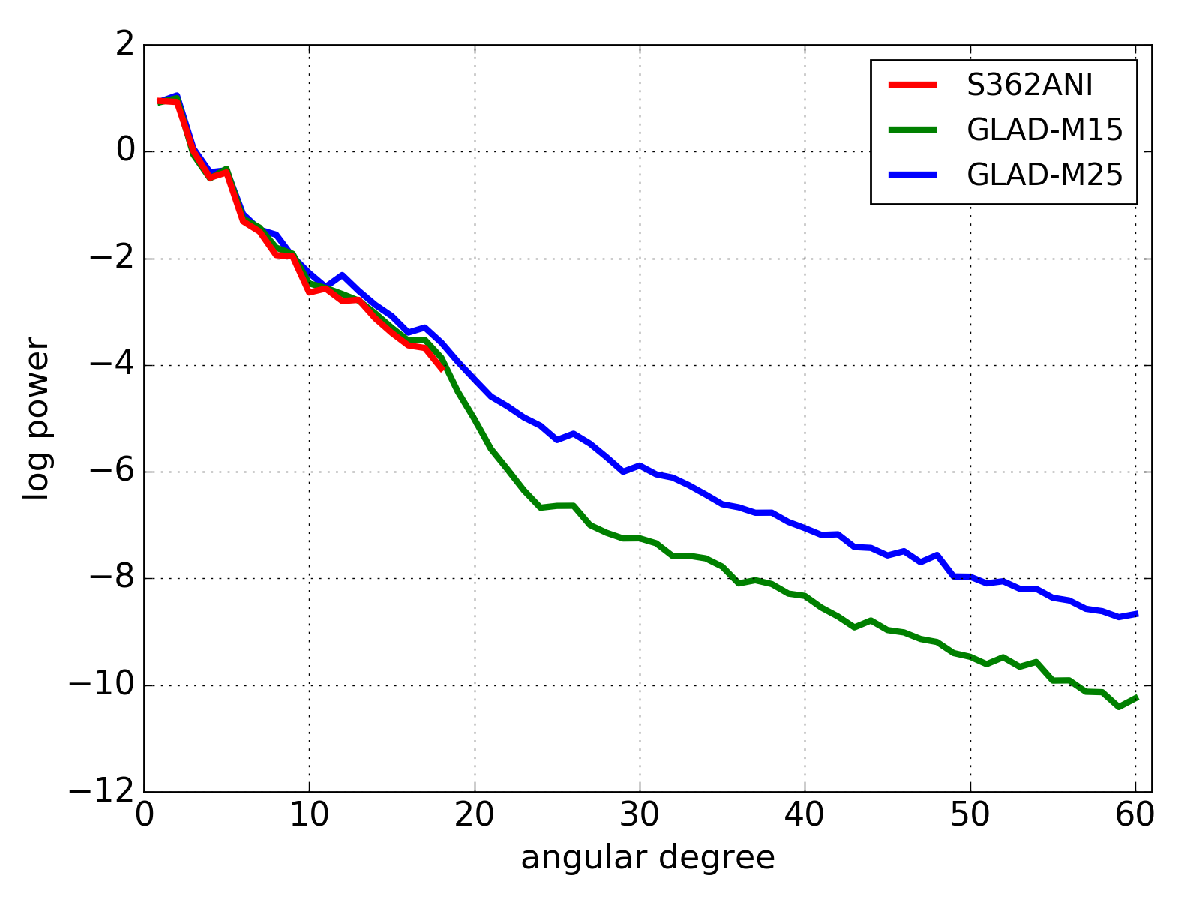
\includegraphics[width=0.5\textwidth]{figures/power.pdf}
  \caption{\small{Normalized power per degree~$\ell$ based on Eqn.~(\ref{eq:powerdegree}), for models S362ANI (red), GLAD-M15 (green), and GLAD-M25 (blue).
  Model S362ANI has no power in degrees greater than~18.
  Included are depths greater than 120~km.
  (Courtesy of Caio Ciardelli.)
  }}
  \label{fig:power}
\end{figure}

\begin{figure}
  \centering
  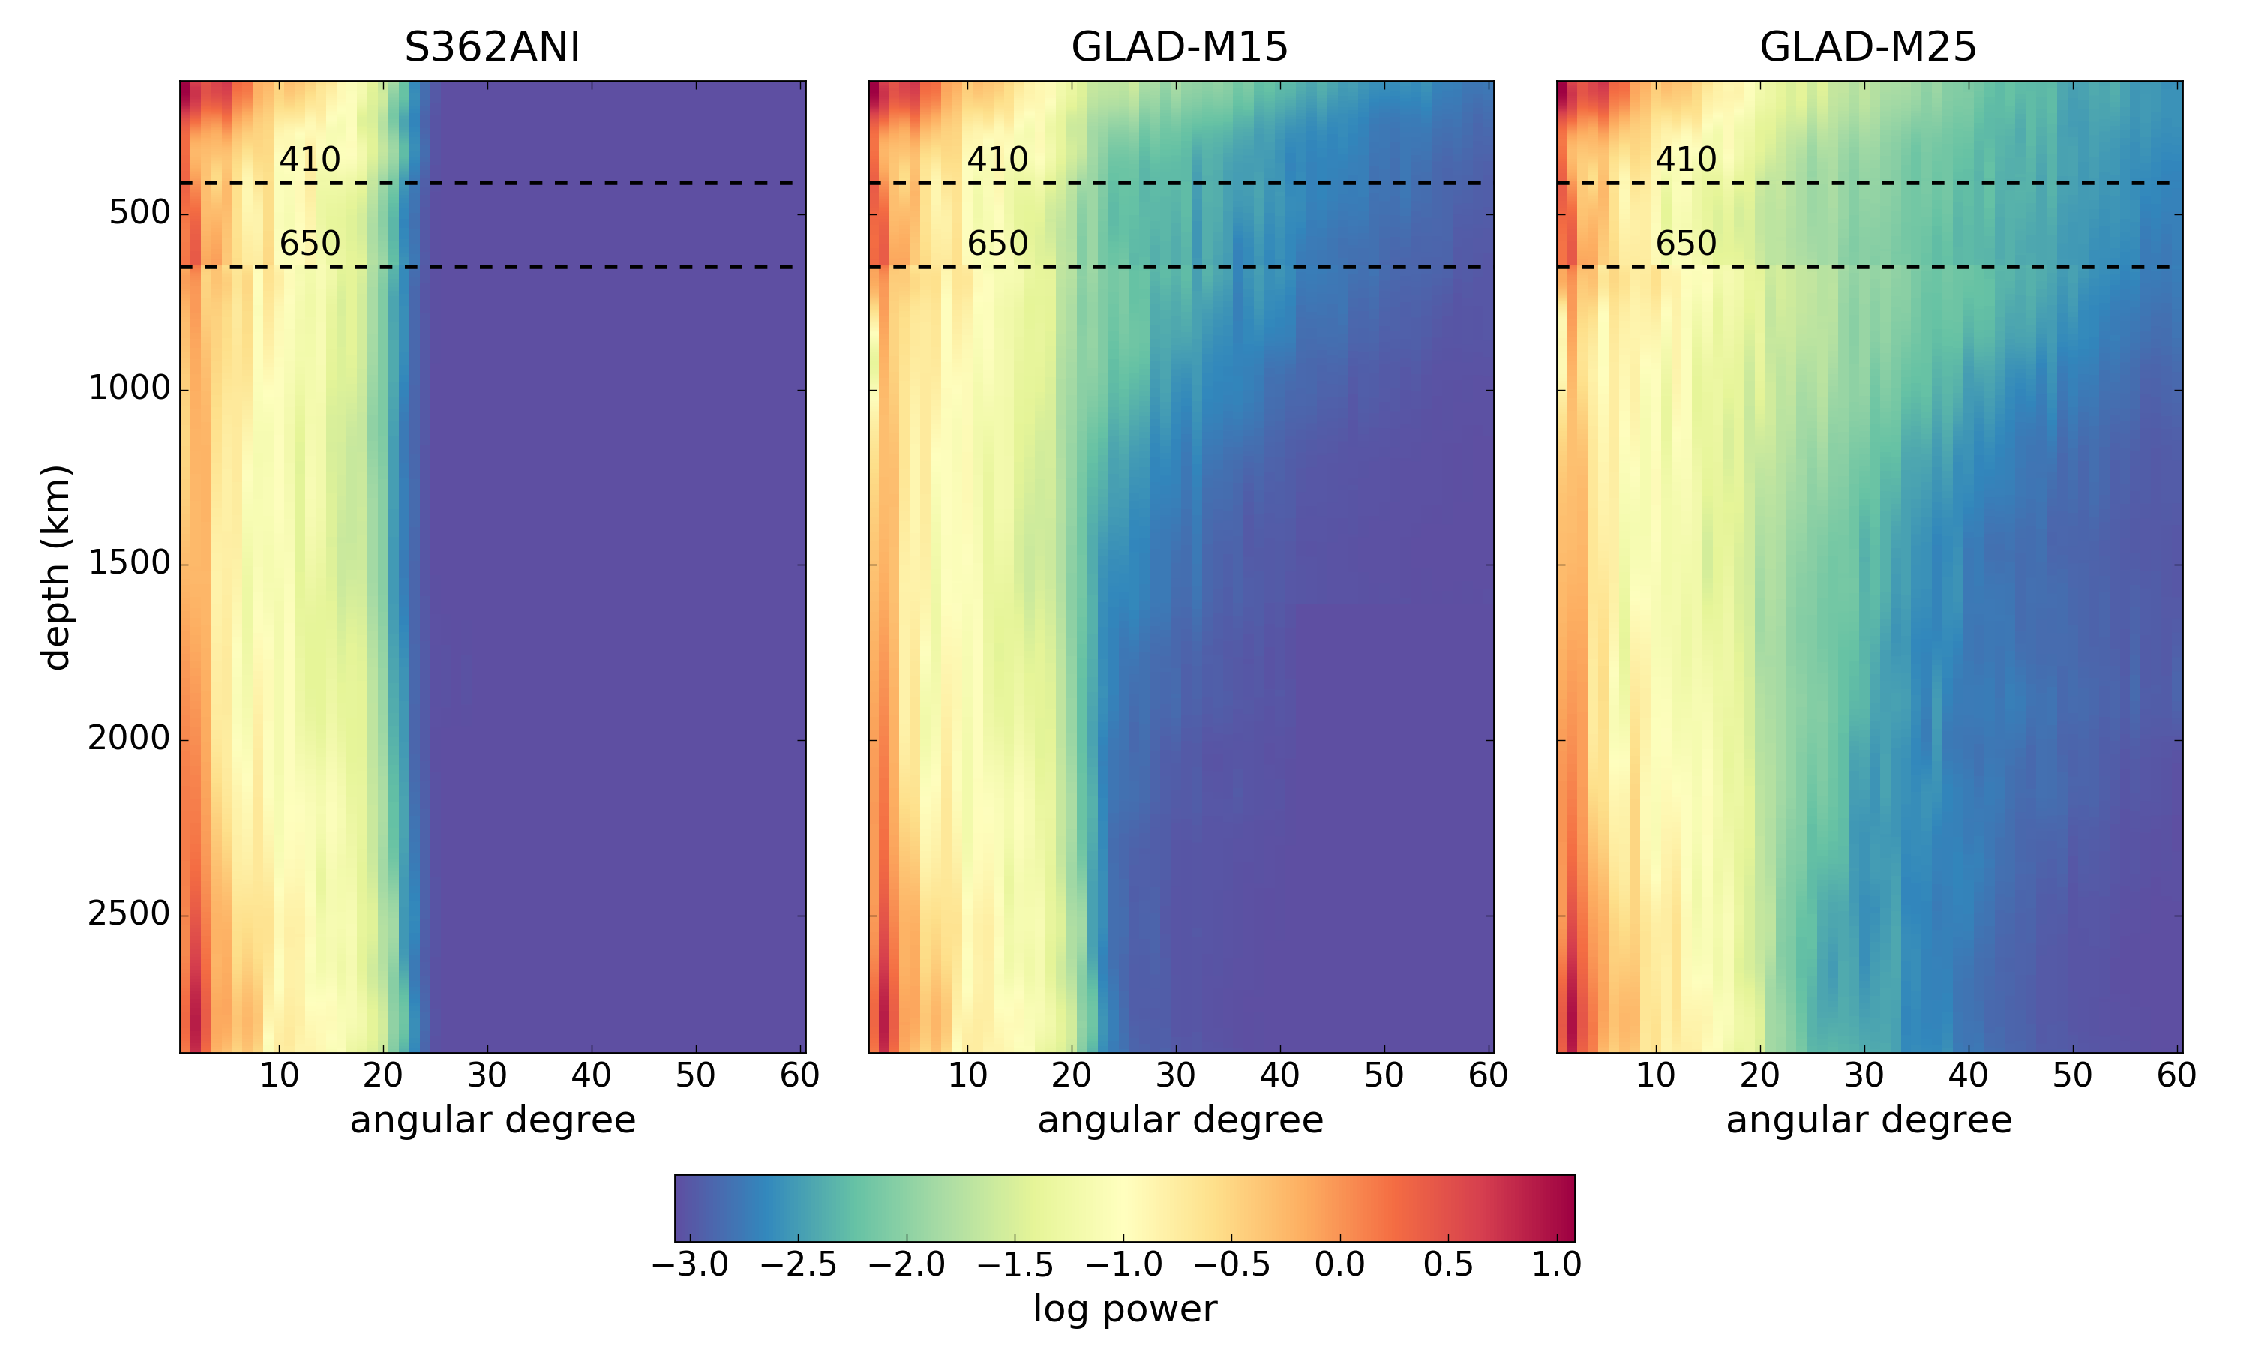
\includegraphics[width=0.95\textwidth]{figures/power_radius.pdf}
  \caption{\small{Normalized power per degree~$\ell$ as a function of radius, based on Eqn.~(\ref{eq:powerdegreeradius}), for models S362ANI (left), GLAD-M15 (middle), and GLAD-M25 (right).
  Shown are depths greater than 120~km.
  (Courtesy of Caio Ciardelli.)
  }}
  \label{fig:powerspectraradius}
\end{figure}

As illustrated in Fig.~\ref{fig:M25-AFAR},
we see an enhancement of the Afar plume relative to GLAD-M15.
The 3D morphology of the African superplume shows a mantle plume rising from the core-mantle boundary with a broad base tilting northward with a thinning neck, before it reaches the 660~km phase boundary and flattens.
It then develops into two sub-plumes ---Afar and East Lake Victoria--- supplying the East Africa rift.
The development of the superplume and its 3D morphology might be associated with water in the mantle transition zone, a possibility we will explore in a future study.

Subduction along the Andes in South America is imaged from south to north all the way down to the transition zone and beyond, as shown in Fig.~\ref{fig:S_America}.
In the contour plot of positive shear-wavespeed perturbations we observe three gaps, which may correspond to ridges or volcanic plateaus on the subducted Nazca plate, and indicate a weakened or even torn slab.

Fig.~\ref{fig:M24-Iceland} showcases the north Atlantic, where we see clear expressions of the Jan Mayen and Iceland plumes as well as the Azores, Canary Islands, and Bermuda,
and Fig.~\ref{fig:M24-Reunion} shows the emergence of hotspots in the Indian Ocean in model GLAD-M25,
including Marion, Crozet, Kerguelen, Cocos, R\'eunion, and Seychelles.

\begin{figure}
  \centering
%  \includegraphics[width=0.9\textwidth]{./figures/M24-AFAR.png}
  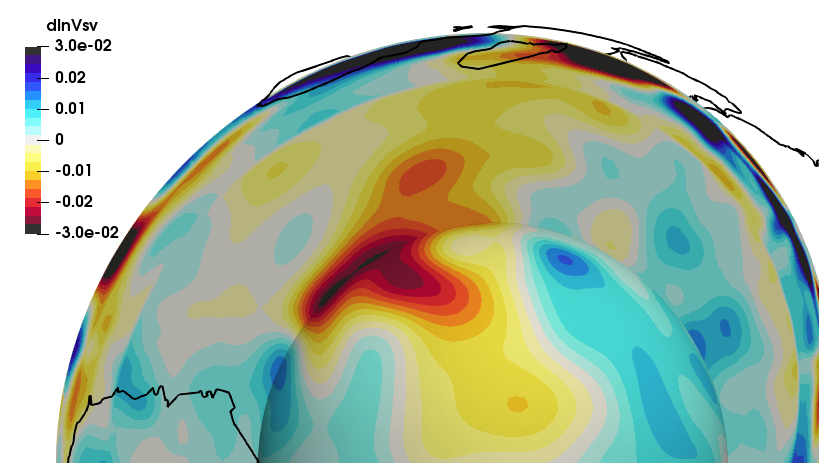
\includegraphics[width=0.45\textwidth]{./figures/afar_M15_dInVsv.png}
  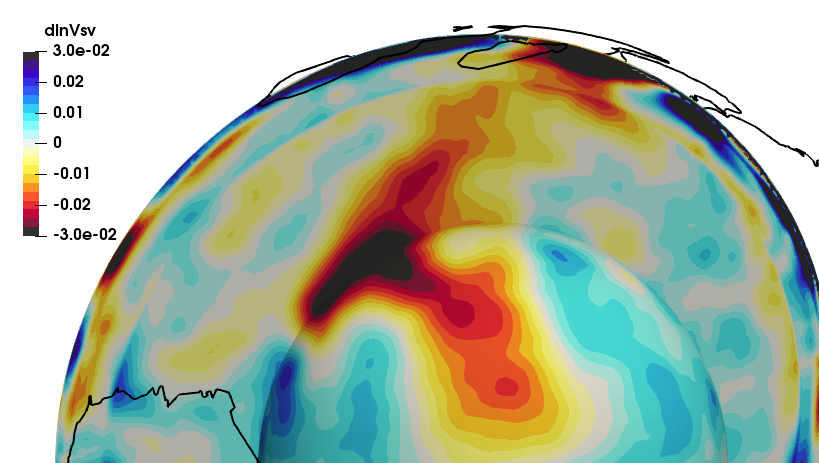
\includegraphics[width=0.45\textwidth]{./figures/afar_M25_dInVsv.png} \\
  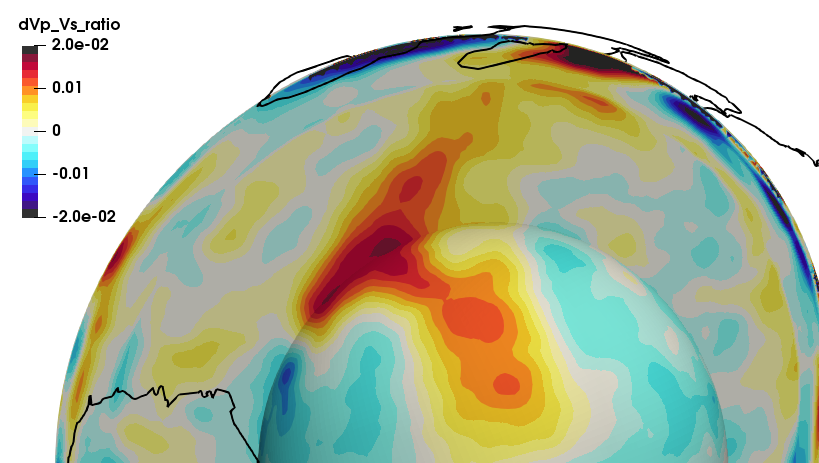
\includegraphics[width=0.45\textwidth]{./figures/afar_M25_dVp_Vs_ratio.png}
  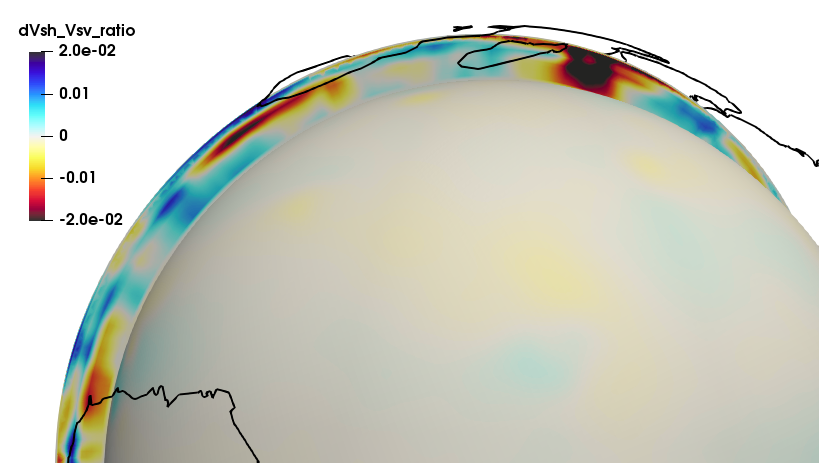
\includegraphics[width=0.45\textwidth]{./figures/afar_M25_dVsh_Vsv_ratio.png}
  \caption{\small{Vertical cross-section of vertically polarized shear-wave-speed $(V_\textrm{SV})$ perturbations ($\pm3$\%) in GLAD-M15 (top left) and GLAD-M25 (top right) underneath Afar. Also shown are $V_\textrm{P}/V_\textrm{S}$ ratios (bottom left) and transverse isotropy (bottom right; $V_\textrm{SH}/V_\textrm{SV}$ ratio) in GLAD-M25 at the same location. In GLAD-M25, the plume becomes larger and more visible, especially in the upper mantle. It also shows how the plume changes its shape when crossing the 660~km discontinuity and ``feeds'' the Afar hotspot at the surface.}}
  \label{fig:M25-AFAR}
\end{figure}

\begin{figure}
\centering
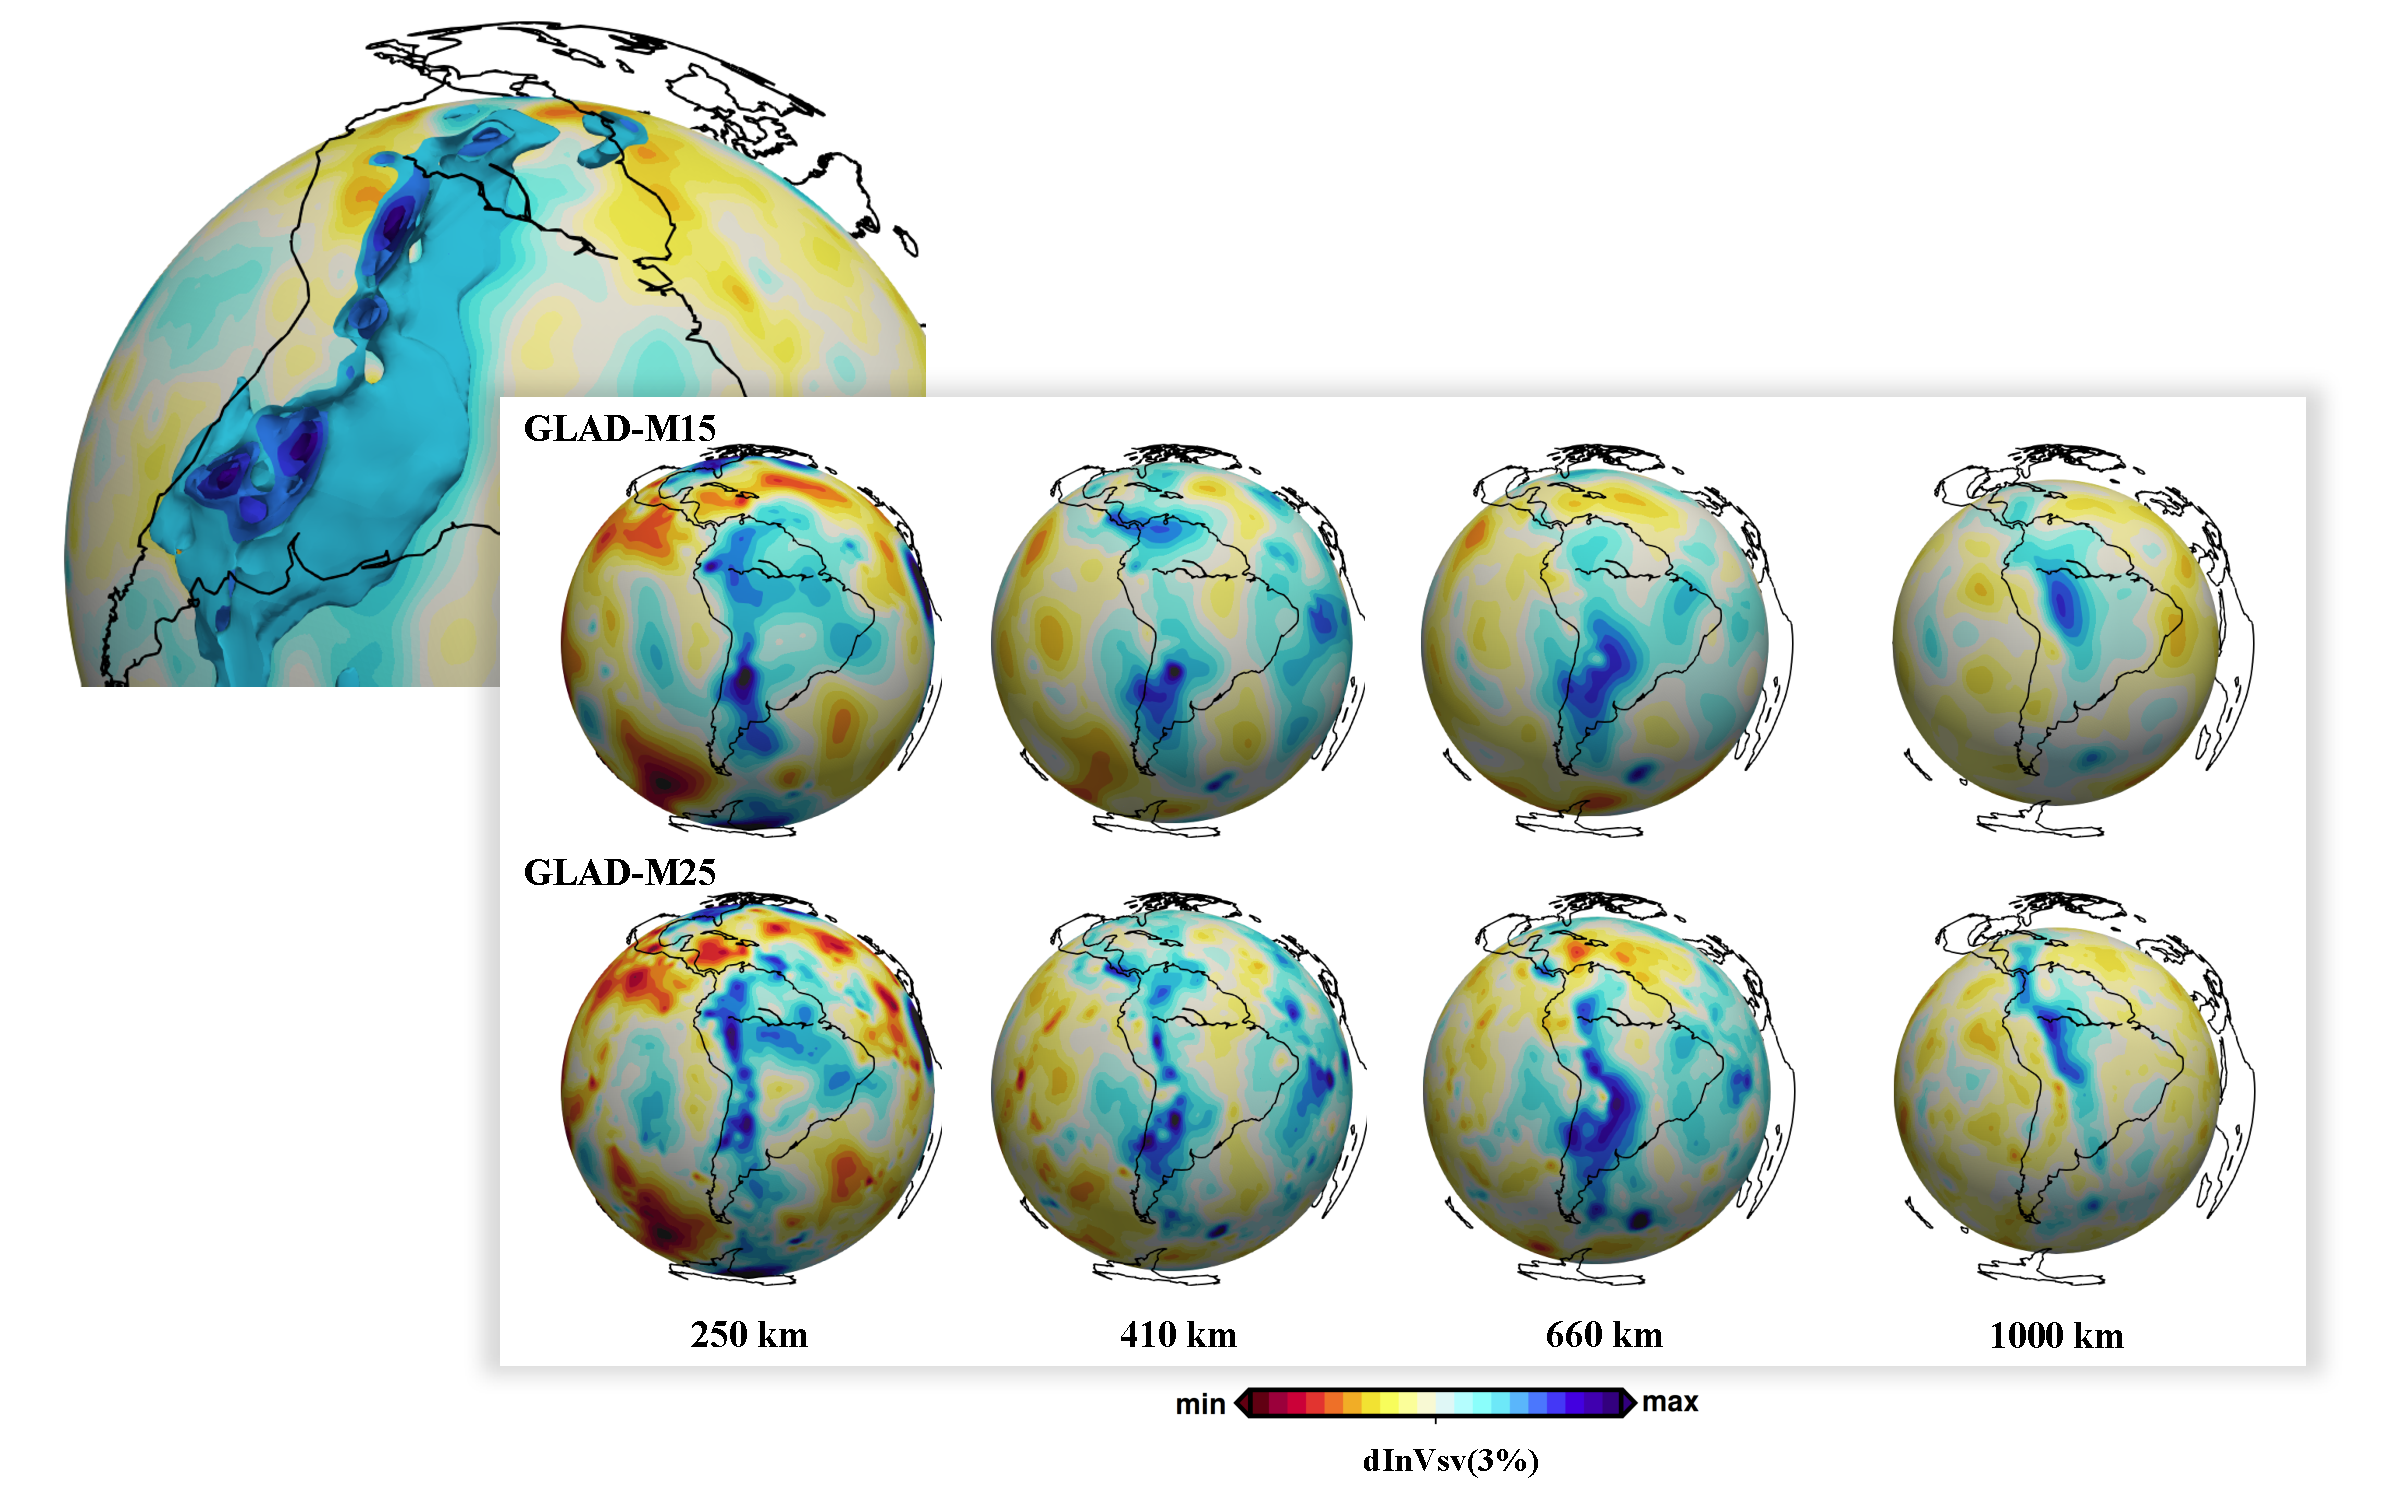
\includegraphics[width=.8\textwidth]{figures/south_america.pdf}
\caption{\small{Contour plot (left) and cross-sections at various depths (right) of subduction underneath South America, showing improvements in resolution in GLAD-M25 compared to GLAD-M15.
The contour plot shows positive perturbations of vertically polarized shear wavespeeds in GLAD-M25. The ball in the contour map denotes the 660~km discontinuity.}}
\label{fig:S_America}
\end{figure}

\begin{figure}
  \centering
  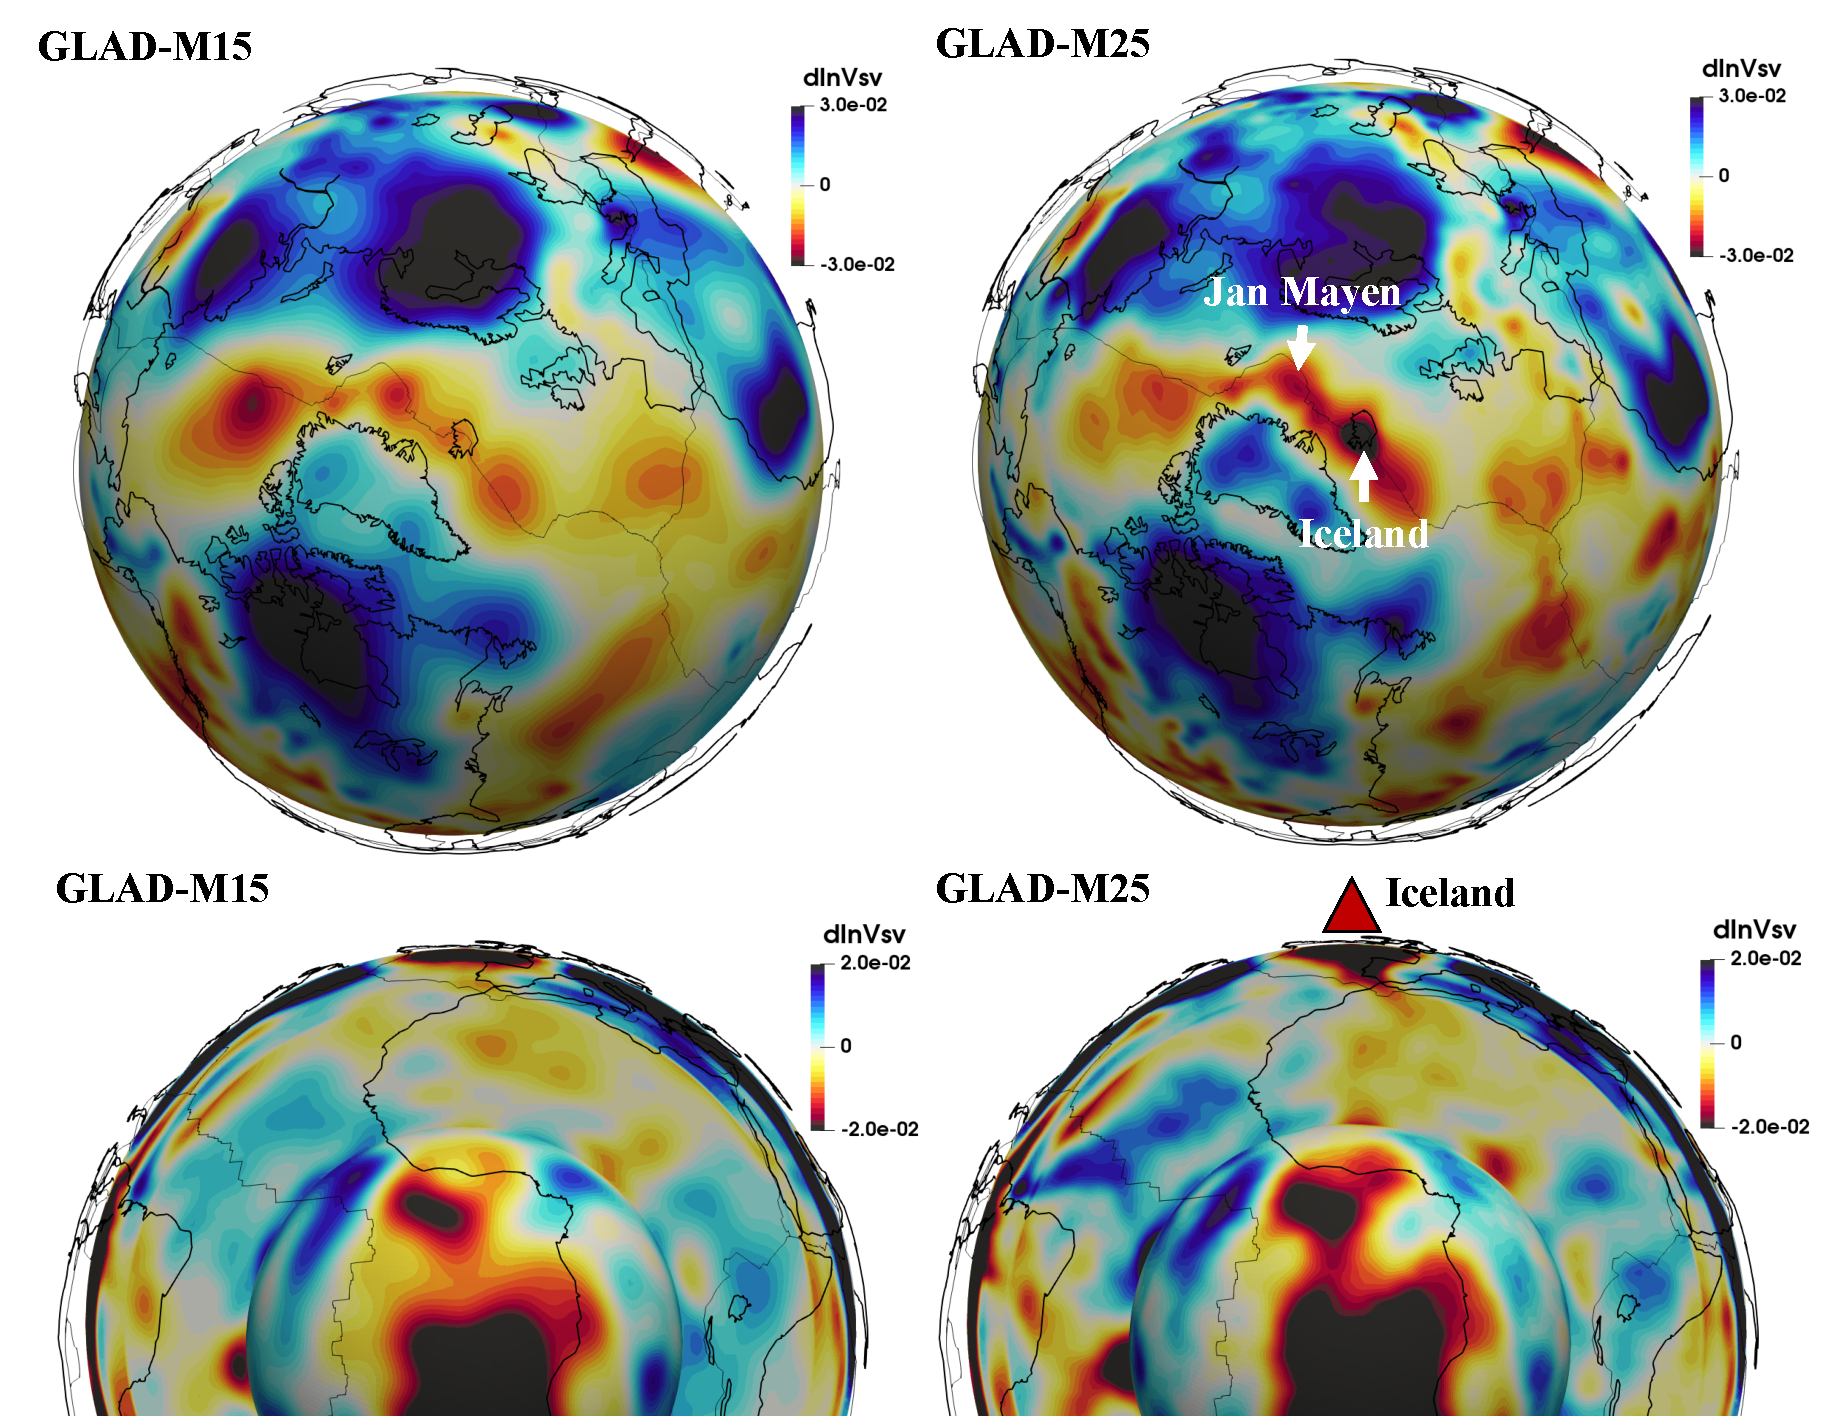
\includegraphics[width=0.8\textwidth]{figures/M25-Iceland.pdf}
  \caption{\small{Map views of vertically polarized shear-wave-speed perturbations in GLAD-M15 (top left) and GLAD-M25 (top right) underneath Iceland. Also shown are vertical cross-sections(bottom row) at the same location. As a primary hotspot, Iceland also becomes more prominent in GLAD-M25, especially in the upper mantle.
  }}
  \label{fig:M24-Iceland}
\end{figure}

\begin{figure}
  \centering
  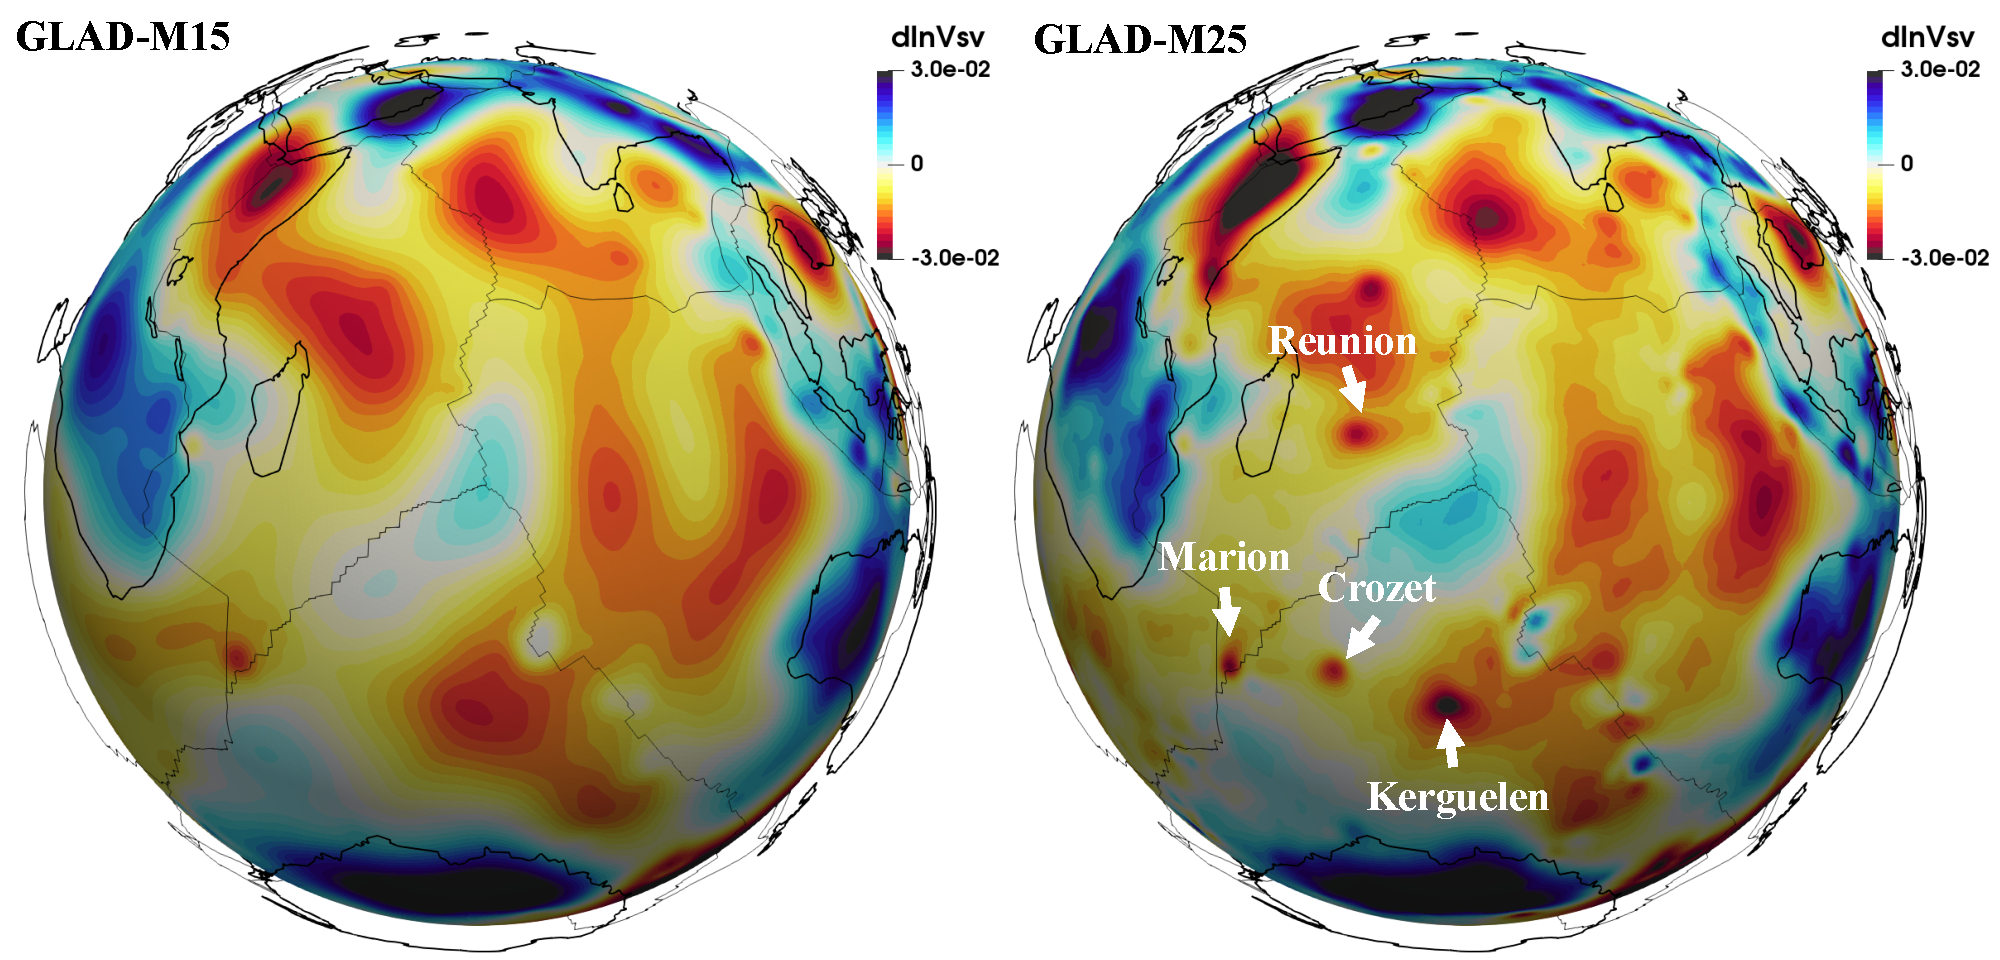
\includegraphics[width=0.8\textwidth]{figures/M25-Reunion.pdf}
  \caption{\small{Map views at 250~km depth of vertically polarized shear-wave-speed perturbations in GLAD-M15 (left) and GLAD-M25 (right) in the Indian Ocean. New features have emerged in GLAD-M25, such as the R\'eunion, Marion, Kerguelen, Maldives, Seychelles, Cocos, and Crozet hotspots.}
  }
  \label{fig:M24-Reunion}
\end{figure}

\subsection{Plumes}
\label{section:plumes}

\begin{figure}
    \centering
    \sidesubfloat[]{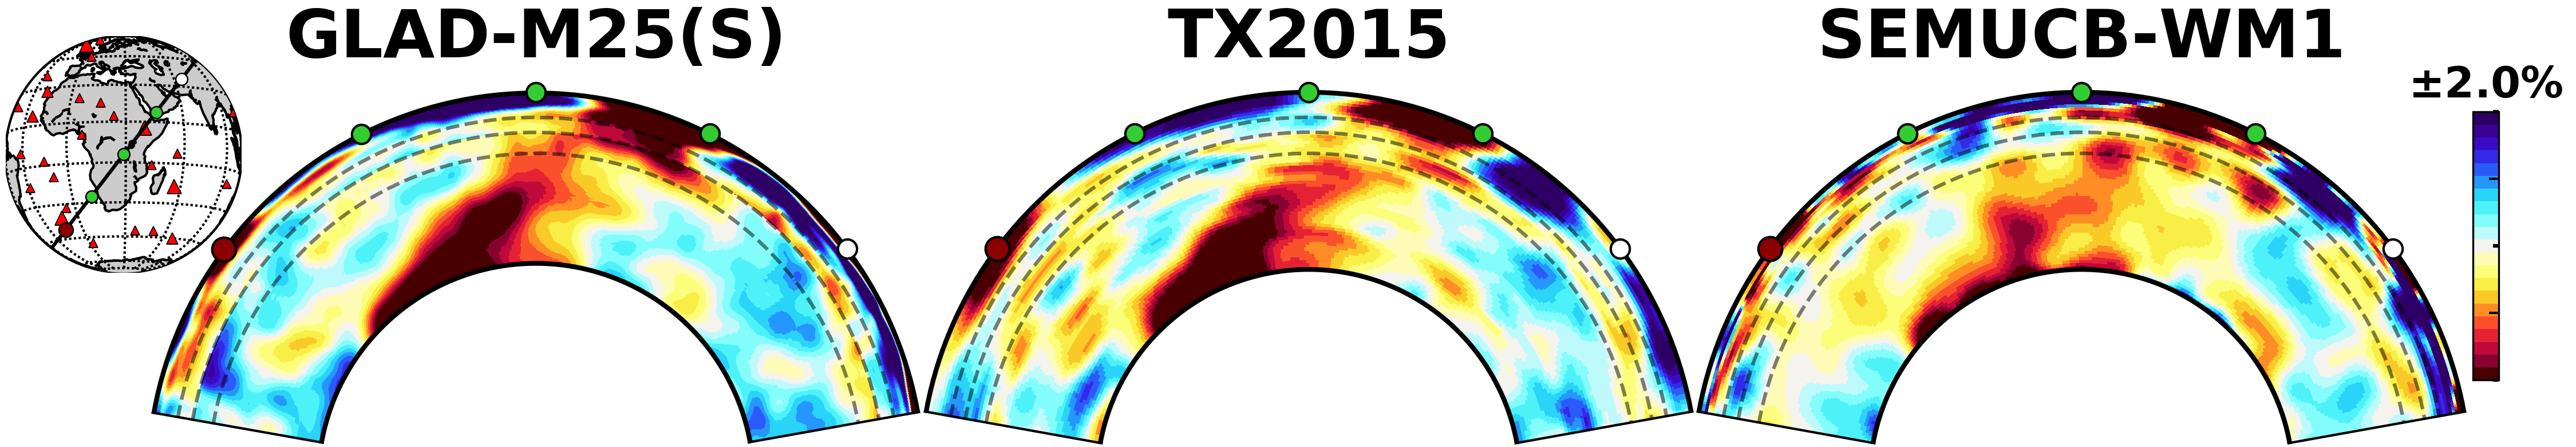
\includegraphics[width=0.98\textwidth]{figures/plumes/Afar.png}}\\[-1pt]
    \sidesubfloat[]{
\includegraphics[width=0.98\textwidth]{figures/plumes/Bermuda_Canary.png}}\\[-1pt]
    \sidesubfloat[]{
\includegraphics[width=0.98\textwidth]{figures/plumes/CapeVerde_Hoggar.png}}\\[-1pt]
    \sidesubfloat[]{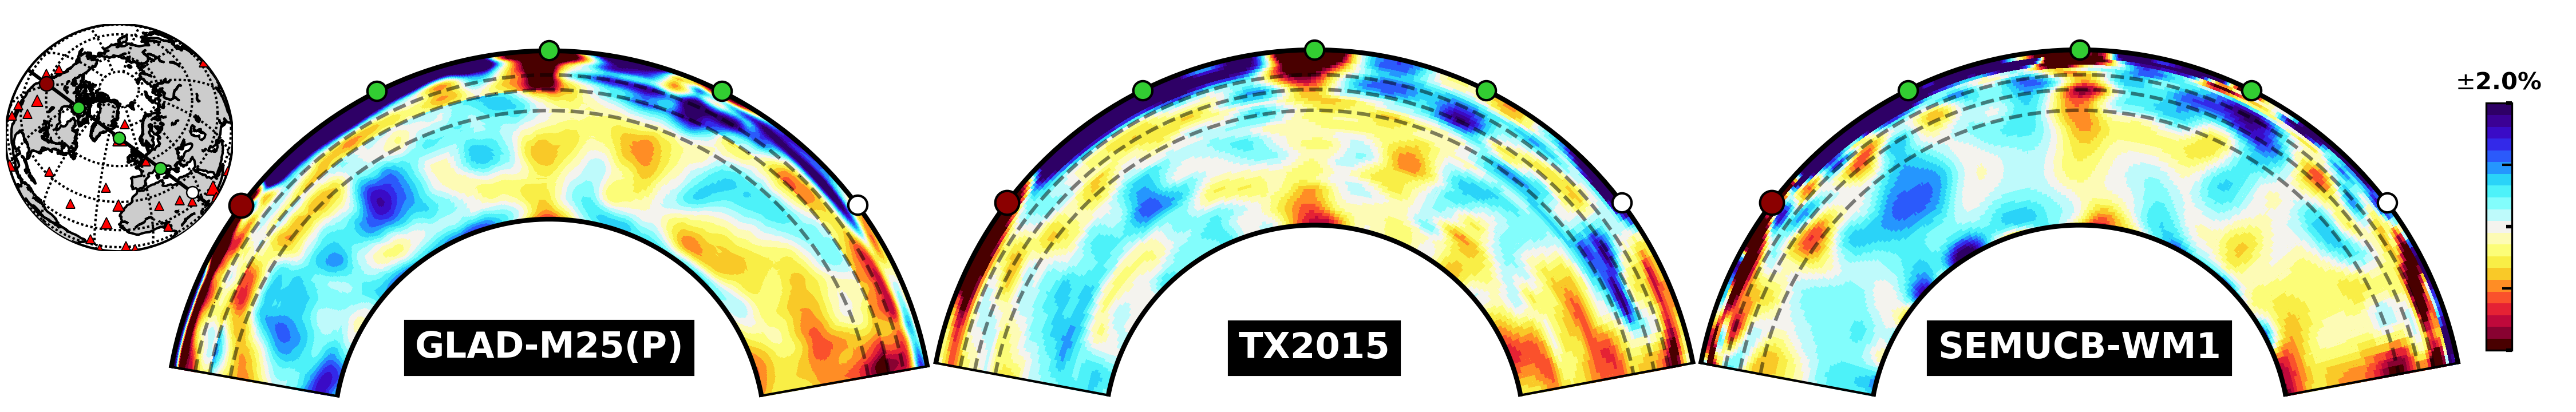
\includegraphics[width=0.98\textwidth]{figures/plumes/Iceland_Eifel.png}}\\[-1pt]
    \sidesubfloat[]{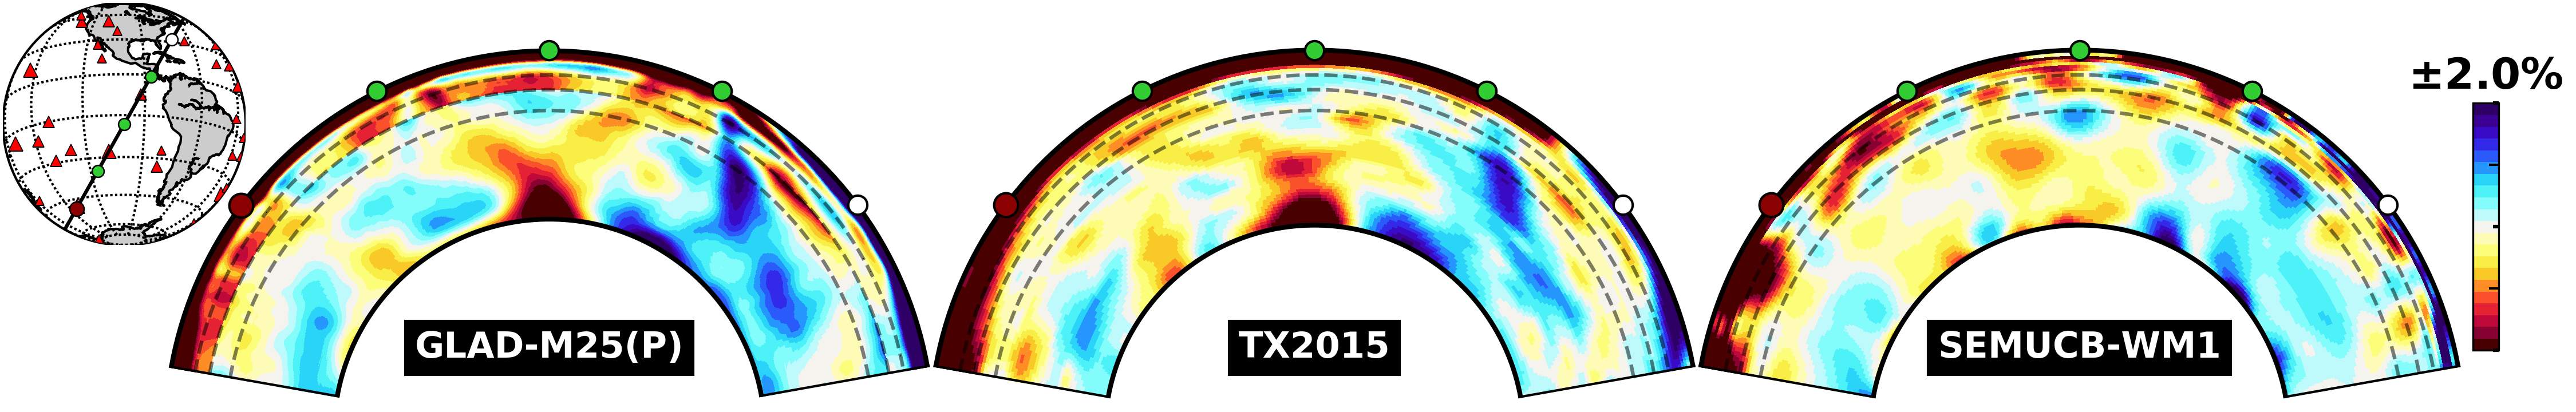
\includegraphics[width=0.98\textwidth]{figures/plumes/Easter_Galapagos.png}}\\[-1pt]
    \sidesubfloat[]{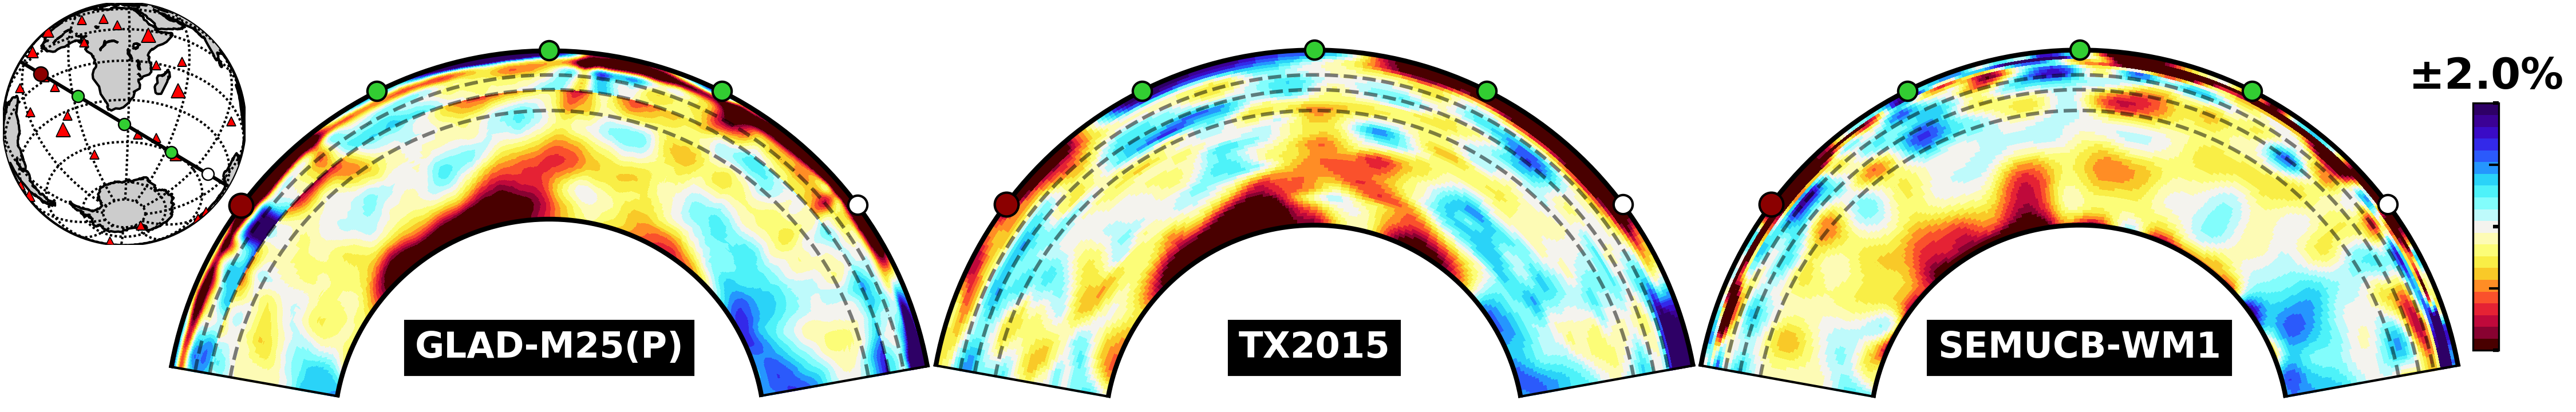
\includegraphics[width=0.98\textwidth]{figures/plumes/Marion3_Kerguelen.png}}\\
    \caption{\small{Vertical cross sections for various plumes for models GLAD-M25 ($V_\textrm{S}$; left column), TX2015~\citep[$V_\textrm{S}$;][]{TX2015} (center column), and SEMUCB-WM1~\citep[$V_\textrm{S}$;][]{french2015broad} (right column).
    The map in the top left corner of each row shows the cross section with color-coded red, green, and white dots for geographical reference;
    hotspots are denoted by red triangles.
    The dashed black semicircles in the cross sections denote depths of 410~km, 660~km, and 1000~km.
    (a) Afar; (b) Bermuda (left) and Canary (middle); (c) Cape Verde (middle) and Hoggar (right); (d) Iceland (middle) and Eifel (right); (e) Easter (left) and Galapagos (right); (f) Marion (middle), and Kerguelen (right). }}
    \label{fig:plumes}
\end{figure}

In this section we highlight various plume systems on Earth. Fig.~\ref{fig:plumes}
shows cross sections of several plumes, comparing models GLAD-M25 ($V_\textrm{S}$),
TX2015~\citep[$V_\textrm{S}$;][]{TX2015}, and SEMUCB-WM1~\citep[$V_\textrm{S}$;][]{french2015broad}.
The three models tend to agree near the CMB,
and there is overall good agreement between GLAD-M25 and TX2015.
The models can differ substantially in the mid and upper mantle,
with different implications for mantle
convection.

\begin{itemize}
\item[]{\it Afar} In Fig.~\ref{fig:plumes}(a),
we see that the Afar plume in model GLAD-M25 originates from the CMB, narrows its diameter
in the mid mantle, and broadens again above the 660~km discontinuity.
It exhibits
very similar behavior in TX2015 but differs significantly in SEMUCB-WM1.  
\item[]{\it Bermuda and Canary} In Fig.~\ref{fig:plumes}(b), from left to right, we see in model GLAD-M25 (i) the Farallon
slab; (ii) the Bermuda hotspot above the 660~km discontinuity; (iii) the Canary hotspot originating from the CMB and
rising all the way up the Earth's surface; (iv) the Afar hotspot from another angle.
\item[]{\it Cape Verde and Hoggar} Fig.~\ref{fig:plumes}(c) features (i) South America subduction; (ii) the Cape Verde hotspot extending from the CMB all the way to the surface; (iii) the Hoggar hotspot from 660~km to the surface. 
\item[]{\it Iceland and Eifel} Fig.~\ref{fig:plumes}(d) shows a plume which rises from the CMB right below Iceland, reaches 660~km, amplifies,
and ascends to the surface.
The intensification above 660~km may be an indication of partial melting.
\item[]{\it Easter and Galapagos} Fig.~\ref{fig:plumes}(e) contains (i) the Easter hotspot; (ii) the Galapagos
hotspot; (iii) the Central America slab.
In models GLAD-M25 and TX2015,
the Easter and Galapagos hotspots appear to originate from the same underlying plume in the deep mantle,
which is the eastern arm of the Pacific superplume.
\item[]{\it Marion and Kerguelen}
Finally,
in Fig.~\ref{fig:plumes}(f) we see the Marion and Kerguelen hotspots, which might be connected to Afar in the lower mantle.
Recovering these plumes is challenging due to poor data coverage in the southern hemisphere.
\end{itemize}

%\begin{figure}
%    \centering
%    \sidesubfloat[]{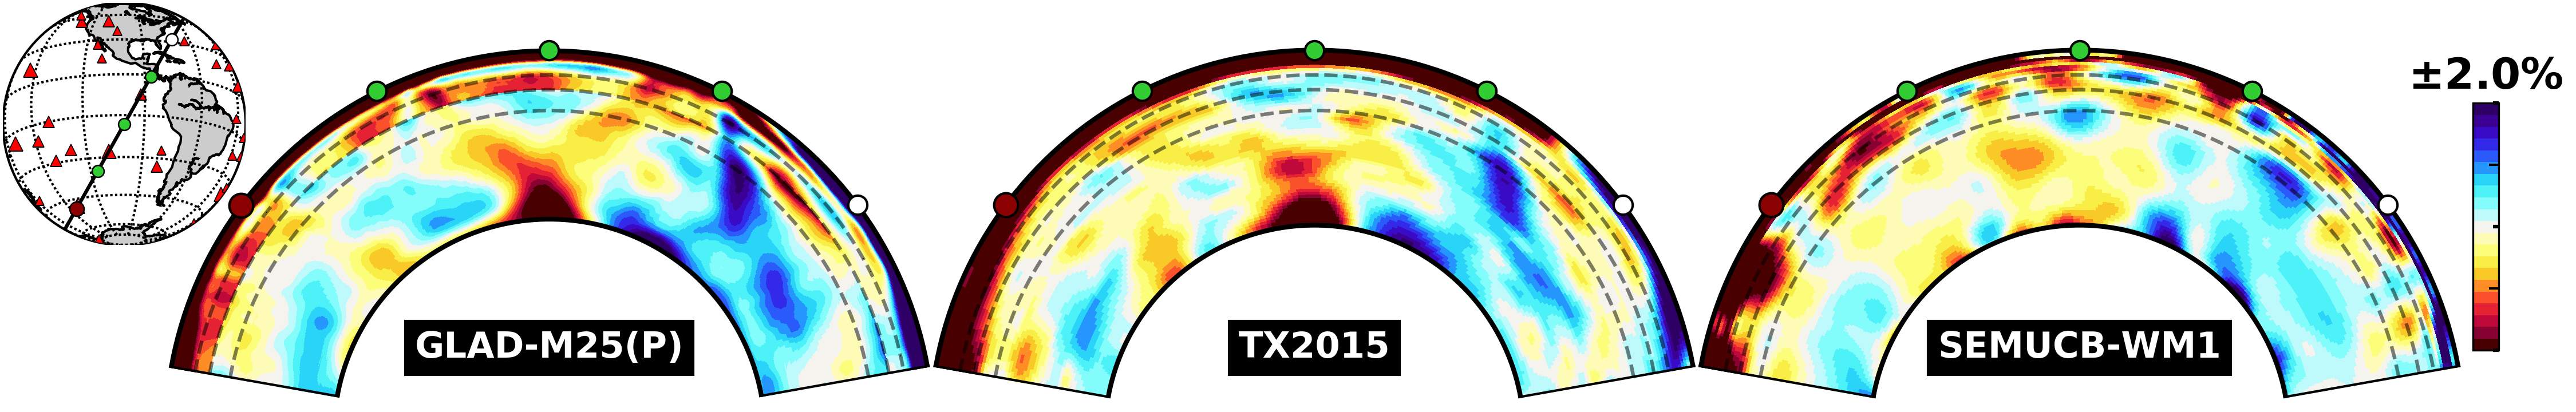
\includegraphics[width=0.98\textwidth]{figures/plumes/Easter_Galapagos.png}\label{fig:a}}\\[-1pt]
%    \sidesubfloat[]{
\includegraphics[width=1.0\textwidth]{figures/plumes/Macdonald_Yellowstone.png}\label{fig:b}}\\[-1pt]
%    \sidesubfloat[]{
\includegraphics[width=1.0\textwidth]{figures/plumes/Pitcairn_Guadalupe.png}\label{fig:c}}\\[-1pt]
%    \sidesubfloat[]{
\includegraphics[width=1.0\textwidth]{figures/plumes/Samoa_Hawaii.png}\label{fig:d}}\\[-1pt]
%    \sidesubfloat[]{
\includegraphics[width=1.0\textwidth]{figures/plumes/Samoa_MarquesasS1.png}\label{fig:e}}\\[-1pt]
%    \sidesubfloat[]{
\includegraphics[width=1.0\textwidth]{figures/plumes/Tahiti_Macdonald.png}\label{fig:f}}\\
%    \caption{\small{Vertical cross sections of shear wave velocity perturbations of plumes in the pacific region.}}
%\end{figure}

\subsection{Subduction zones}
\label{section:slabs}

\begin{figure}
    \centering
    \sidesubfloat[]{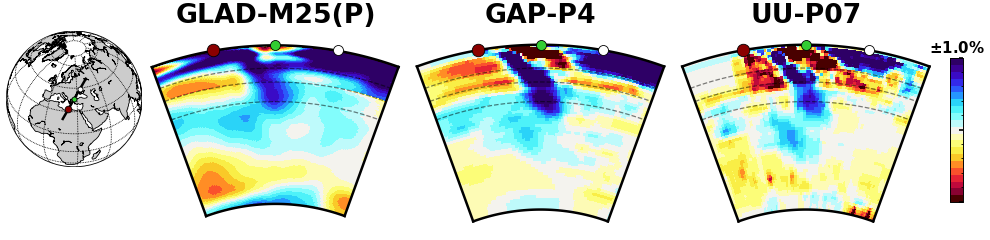
\includegraphics[width=0.88\textwidth]{figures/subductions/Aeg.png}\label{fig:subd_a}}\\[-8pt]
    \sidesubfloat[]{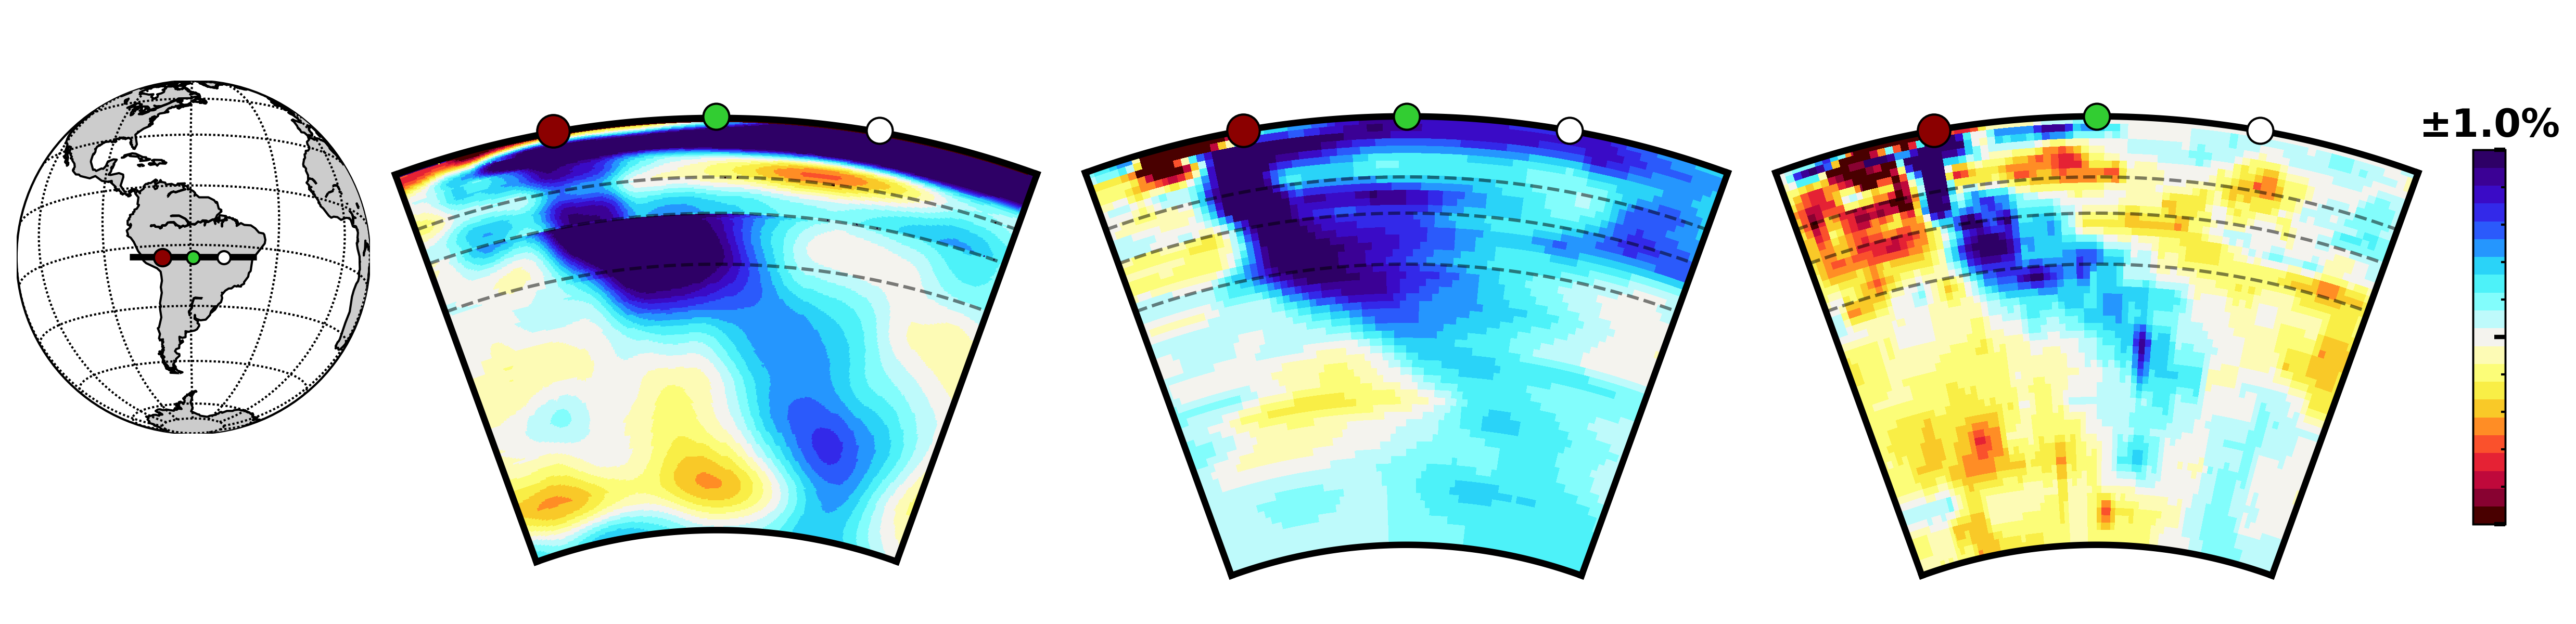
\includegraphics[width=0.88\textwidth]{figures/subductions/Br.png}\label{fig:subd_b}}\\[-8pt]
    \sidesubfloat[]{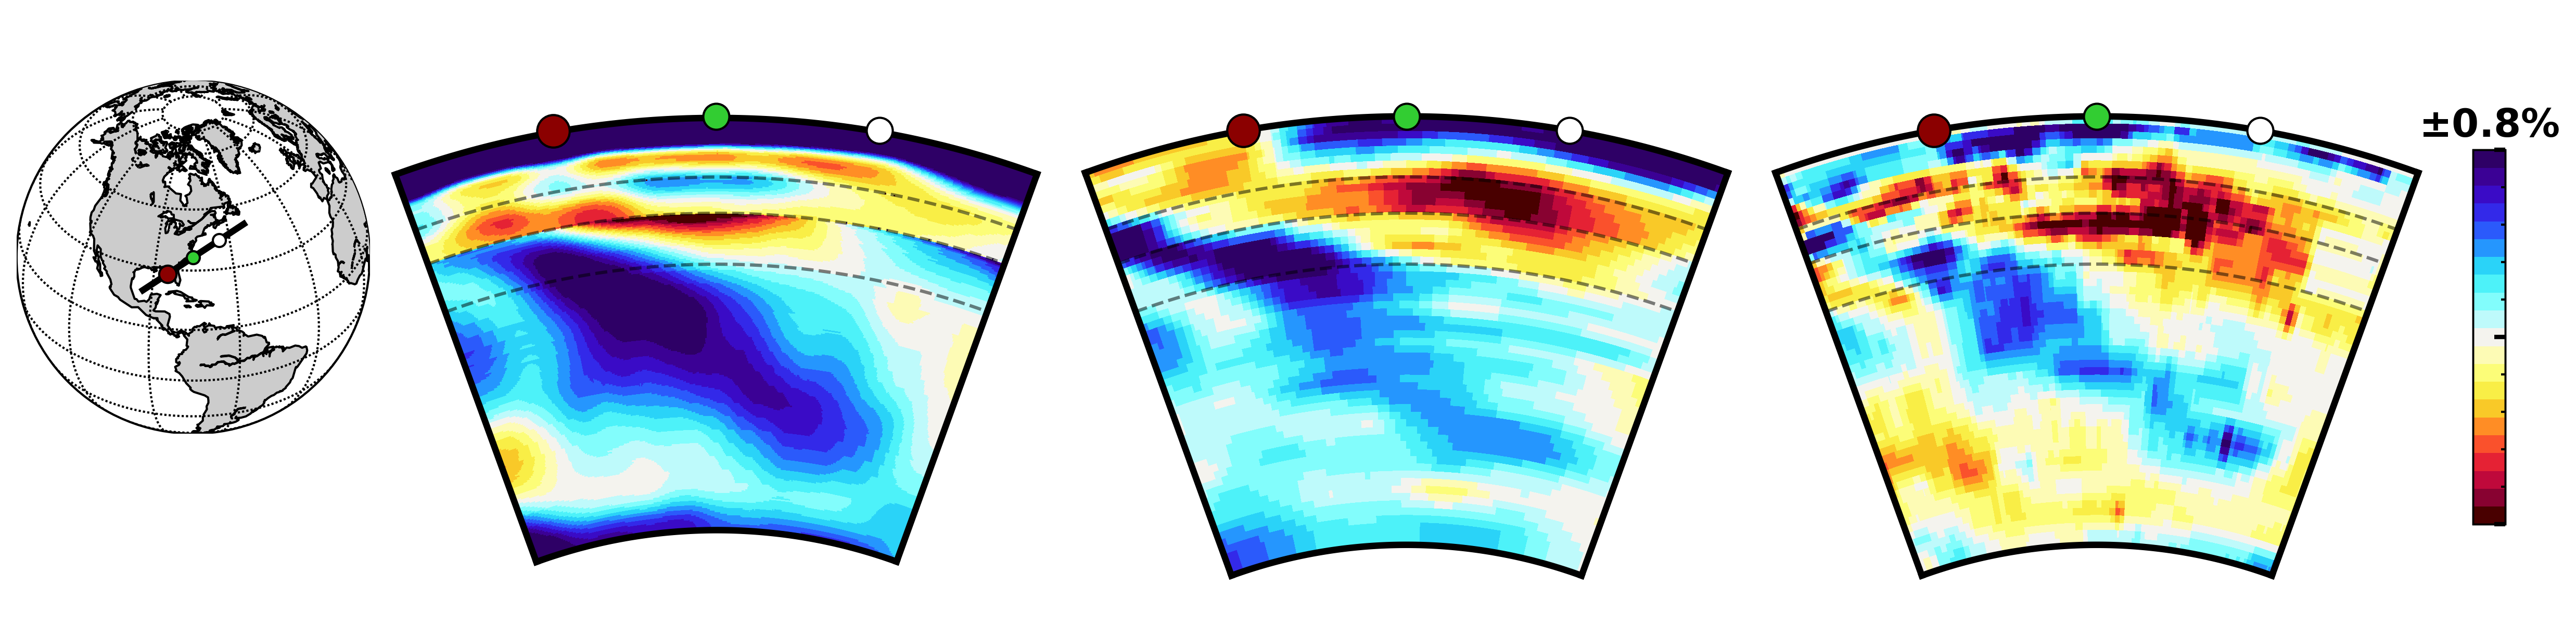
\includegraphics[width=0.88\textwidth]{figures/subductions/Ha.png}\label{fig:subd_c}}\\[-8pt]
    \sidesubfloat[]{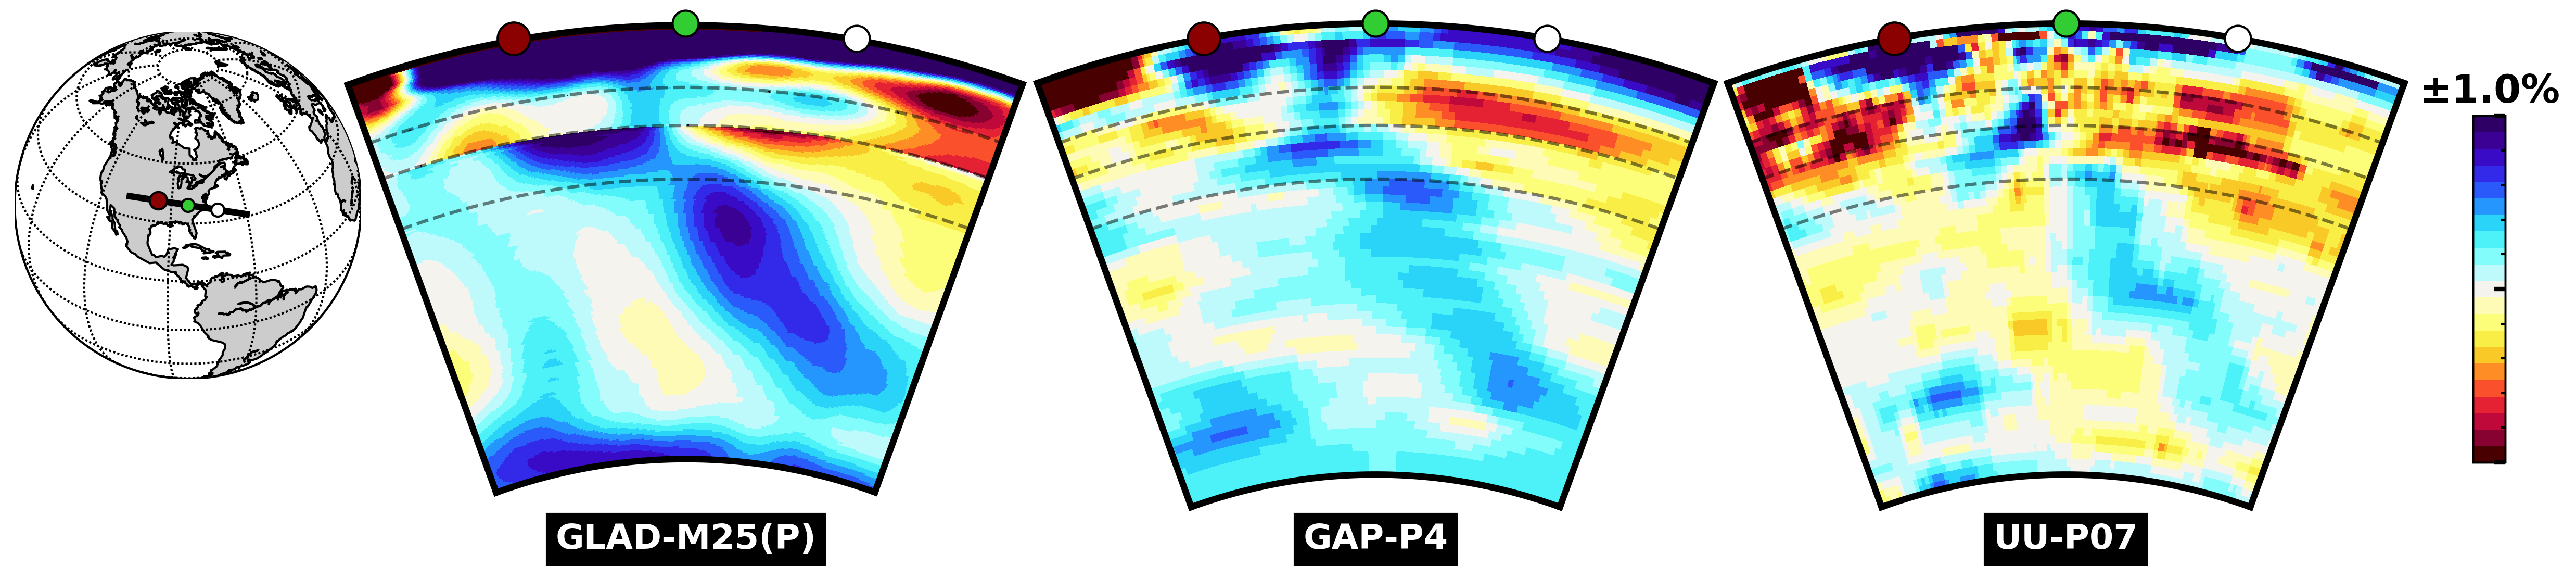
\includegraphics[width=0.88\textwidth]{figures/subductions/Wc.png}\label{fig:subd_e}}\\[-8pt]
    \sidesubfloat[]{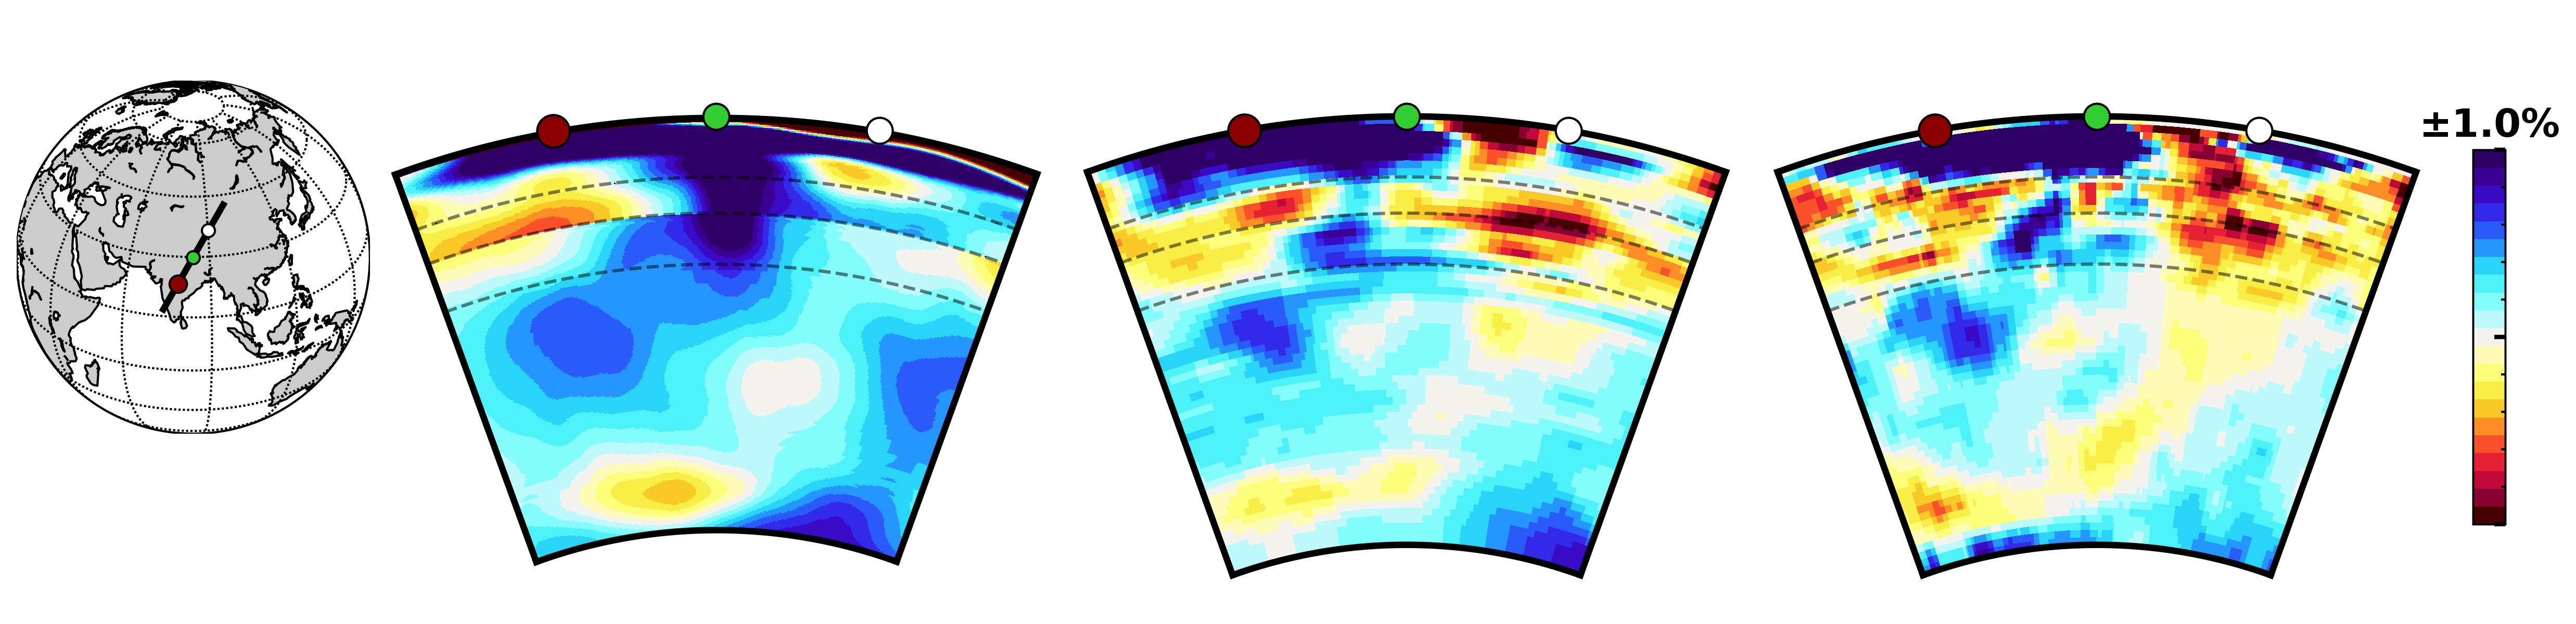
\includegraphics[width=0.88\textwidth]{figures/subductions/Ne.png}\label{fig:subd_d}}\\[-8pt]
    \sidesubfloat[]{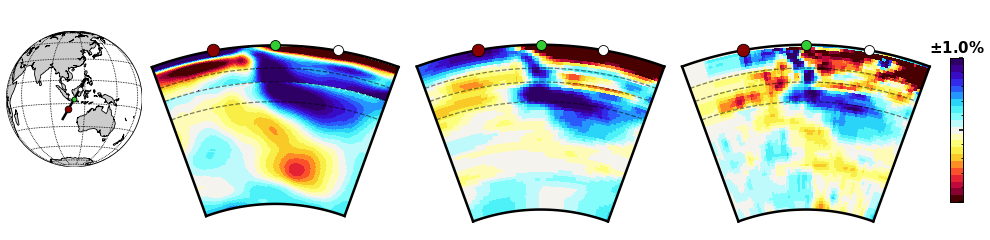
\includegraphics[width=0.88\textwidth]{figures/subductions/Su.png}\label{fig:subd_f}}\\[-8pt]
    \caption{\small{Vertical cross sections of compressional wavespeed perturbations in various subduction zones
    for models GLAD-M25 ($V_\textrm{P}$; left column), GAP-P4~\citep{fukao2013subducted} (middle column) and UU-P07~\citep{van2018atlas} (right column).
    The map in the top left corner of each row shows the cross section with color-coded red, green, and white dots for geographical reference.
    The dashed black semicircles in the cross sections denote depths of 410~km, 660~km, and 1000~km.
    (a) Aegean; (b) South America; (c) Hatteras; (d) Wichita. (e) Nepal; (f) Sunda. }}
    \label{fig:subd}
\end{figure}

In this section we highlight various subduction systems on Earth.
In Fig.~\ref{fig:subd} we compare GLAD-M25~($V_\textrm{P}$) with two compressional wavespeed models,
namely, GAP-P4~\citep{fukao2013subducted} and UU-P07~\citep{van2018atlas}.
Fig.~\ref{fig:subd}(a) features the Aegean subduction zone. All models show a slab penetrating into the lower mantle beyond a depth of 1,000~km.
Fig.~\ref{fig:subd}(b) shows the South American slab, which, in this cross section, ponds in the shallow lower mantle in all three models, before sinking all the way to the CMB.
Figs.~\ref{fig:subd}(c) and~(d) show cuts across the ancient Farallon slab, which penetrates deeply into the lower mantle,
as documented by, for instance, \citet{grand1994}, \cite{hilst1997}, and \cite{grand1997high}.
At depths greater than 1,000~km, 
we see a very strong expression of the slab in model GLAD-M25, which is much weaker in the two P models.
The difference may be attributed to increased data coverage thanks to USArray, as well as the use of finite-frequency Fr\'echet derivatives.
Fig.~\ref{fig:subd}(e) shows subduction beneath the Himalayas.
All three models show two distinct fast anomalies below 660~km,
one above 1,000~km and the other, further to the southwest, below 1,000~km.
Finally, Fig.~\ref{fig:subd}(f) shows subduction beneath the Java portion of the Sunda Arc.
At this location the slab penetrates into the lower mantle, at which point its spreads out laterally,
in agreement with models GAP-P4 and UU-P07.
\cite{fukao1992} explained this flattening using a model of~\cite{ringwood1988},
suggesting that the subducted slab thickened and buckled to form a dense megalith
above the 660~km discontinuity before sinking into the lower mantle.

Overall, the three models are in reasonably good agreement.
At shallow depths, model GLAD-M25 shows more distinct continental crust and cratons, thanks to the inclusion of surface waves.
But in the upper and mid mantle,
the models share similar attributes.

\section{Discussion}

As illustrated in Figs.~\ref{fig:window_density_Z}, \ref{fig:window_density_R}, and~\ref{fig:window_density_T},
the goal of our inversion is to assimilate as much seismic waveform information as possible.
To facilitate fast and effective assimilation of such data,
we use the Adaptable Seismic Data Format~\citep{krischer2016adaptable} in the preprocessing stage of the adjoint tomography workflow,
and to accommodate I/O during the postprocessing stage we use the ADIOS library~\citep{liu2014hello}.
For data assimilation,
tools such as FLEXWIN, which automatically select data windows suitable for measurements, are indispensable, and we see opportunities for the use of machine learning algorithms in this context~\citep[e.g.,][]{chen2017}.
Without these libraries and tools, the construction of model GLAD-M25 would have been impossible. 

Some form of automated parallel workflow management is critical for the global adjoint tomography process,
because classical inversion workflows suffer from I/O inefficiencies, lack of fault tolerance, and an inability to work in distributed resource environments~\citep{Lefebvre2018}.
For these reasons, we are in the process of adopting the Ensemble Tool Kit (EnTK) as our
workflow management engine~\citep{EnTK2017}.
This workflow engine can automatically detected job failures,
both from the high-performance computing (HPC) system and via user-defined functions.
This facilitates tracking of tasks and semi-automatic job resubmission if necessary.
These are the attributes required for bringing global FWI to its full potential,
enabling the assimilation of data from thousands of earthquakes on the largest HPC systems.

It should be clear from this discussion that modern seismic tomography requires close collaborations with computational scientists, HPC specialists, and visualization experts,
as reflected in the list of authors for this article, in addition to access to advanced computational platforms,
such as those offered through the DOE INCITE and NSF XSEDE programs.

Although Figs.~\ref{fig:window_density_Z}--\ref{fig:window_density_T} illustrate that much information in seismograms is
being assimilated, we still have a long way to go before explaining every broadband wiggle in hundreds-of-minutes-long seismograms.
Currently, we are only fitting the phase in selected time windows, and amplitude information remains completely unused.
We accommodate the full physics of seismic wave propagation,
but we are not exploiting the most general earth model parameterization.
GLAD-M25 is an elastic model with radial anisotropy confined to the upper mantle.
It is well known that the upper mantle is azimuthally anisotropic~\citep[e.g.,][]{montagner1989petrological,montagner1991},
and we also know that amplitude information helps constrain second derivatives in phase speed~\citep[e.g.,][]{WW86,TDI,TDII},
in addition to lateral variations in attenuation~\cite[e.g.,][]{romanowicz1998,reidetal2001,DaEkDz08}.
Thus, the natural next step in global FWI is to use phase and amplitude information simultaneously to jointly constrain the elastic and anelastic structure of the Earth.
To accomplish this next step, source parameters need to be constrained more precisely, especially as we push the resolution to shorter periods~\citep[e.g.,][]{valentine2010}.

The global distribution of earthquakes and stations is highly uneven (Fig.~\ref{fig:eventsstations}).
This problem may be alleviated to some extent by using suitably chosen misfit functions with appropriate geographical weighting of sources and receivers~\citep[e.g.,][]{Li1996,Ruanetal2018}.
The ultimate solution may be a dense network of Ocean Bottom Seismometers,
but meanwhile an armada of floating seismometers may offer a cheaper and more practical alternative~\citep[e.g.,][]{Nolet19}.

\section{Conclusion}

Building on our experiences during the construction of our first-generation global adjoint tomography model GLAD-M15~\citep{bozdaug2016global},
for this study we expanded our earthquake database from 253 to 1,480 events,
which were collectively recorded by more than 11,000 seismographic stations.
We used three-component seismograms in four period bands,
namely 17--40~s body waves, 40--100~s body waves, 40--100~s surface waves, and 90--250~s surface waves,
resulting in twelve measurement categories.
This culminated in the assimilation of more than 18~million time windows.

GLAD-M25 --- like its predecessor GLAD-M15 --- invokes no crustal corrections, and constrains crust and mantle shear and compressional wavespeeds simultaneously.
Such ubiquitous crustal corrections may affect inferences about upper-mantle anisotropy~\citep[e.g.,][]{BozdagTrampert2008,PaLeRo10,Ferreira10}, and are likely the main reason for significant differences between radially anisotropic upper-mantle models~\citep[e.g.,][]{Chang14}.
Treating the crust and mantle equally and simultaneously is one of the main strengths of GLAD-M25, accepting the additional computational costs, but thereby avoiding any approximations or corrections.
Another strength is the fact that the effects of attenuation are fully accommodated, both in forward and in adjoint simulations.
These points highlight the importance of taking the full physics of seismic wave propagation properly into account in seismic imaging. 

Another attribute of GLAD-M25 is that it constrains shear and compressional wavespeeds simultaneously in the same period range,
thereby enabling us to interpret the two wavespeeds together.
As illustrated in Figs.~\ref{fig:window_density_Z} and~\ref{fig:window_density_R},
numerous compressional wave arrivals are assimilated, including P, PP, PPP, PKP, PS, and PPS.
In future work we will capitalize on this by using the $V_\text{P}/V_\text{S}$ ratio to help constrain thermo-chemical and geodynamical processes in the mantle.

GLAD-M25 was quantitatively evaluated in several ways.
First, it produces 14.4--33.6\% (relative to GLAD-M15) and 37.3--77.2\% (relative to S362ANI combine with CRUST2.0) variance
reductions in twelve measurements categories.
Second,
it produces reasonably well centered Gaussian traveltime anomaly histograms
in all measurement categories.
Third, point-spread function tests show minimal tradeoffs between model parameters and reasonably good resolution in the frequency band of interest.
Finally,
for a held-out data set of 360 events
we see similar misfit reductions and traveltime anomaly histograms as in the actual inversion.

When we compare GLAD-M25 with other global models,
we find overall good agreement at longer wavelengths.
In particular, GLAD-M25 and TX2015 feature similar plume structures.
However, even in regions with dense seismographic coverage, such as North America,
recent models can differ substantially, especially at greater depths.
Nevertheless, our global inversion is bridging the gap between global and regional studies,
approaching regional-scale resolution is areas with sufficient data coverage.
We can observe this increase in resolution in GLAD-M25 in the normalized power per spherical harmonic degree as a function of radius (Fig.~\ref{fig:powerspectraradius}).


% \begin{figure}
%   \centering
%   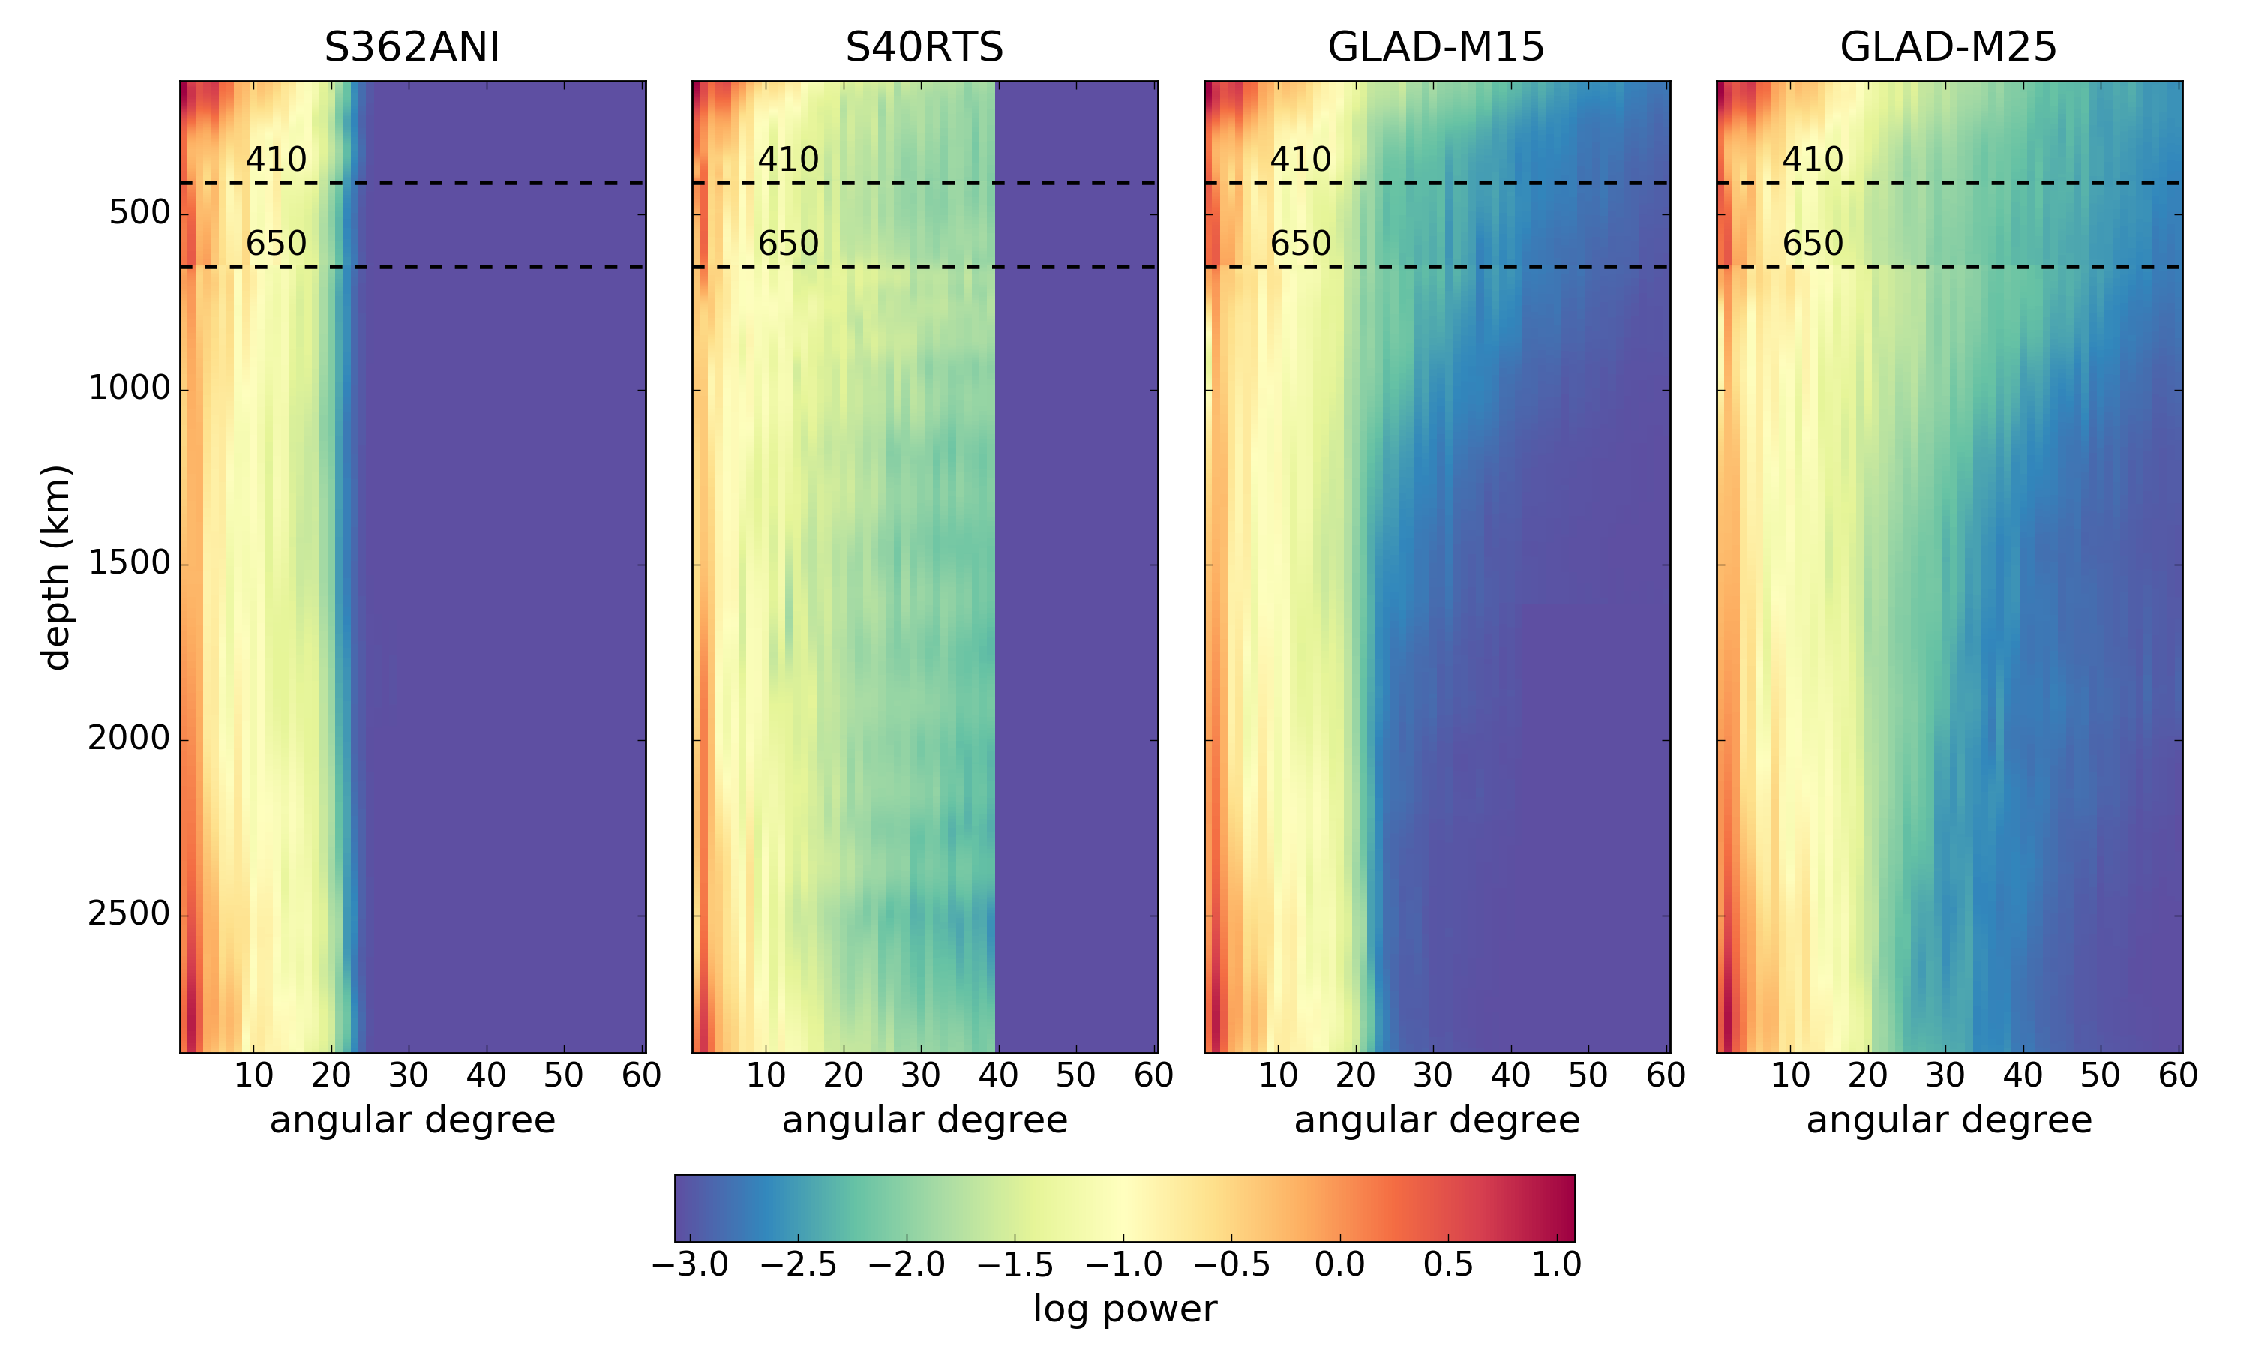
\includegraphics[width=0.95\textwidth]{figures/power_radius2.pdf}
%   \caption{\small{Normalized power per degree~$\ell$ as a function of radius, based on Eqn.~(\ref{eq:powerdegreeradius}), for models S362ANI (first column), S40RTS (second column), GLAD-M15 (third column), and GLAD-M25 (fourth column).
%   Shown are depths greater than 120~km.
%   (Courtesy of Caio Ciardelli.)
%   }}
%   \label{fig:powerspectraradius}
% \end{figure}

Obvious future directions of research include growing the earthquake database further to the roughly 6,000 earthquakes in the right magnitude range already available via the Global CMT database,
and reducing the shortest simulation period further from 17~s to 9~s.

Other future directions of research involve inversions for azimuthal anisotropy
and attenuation.
The feasibility of such inversions on a regional scale has already been demonstrated in studies focused on Europe by~\cite{ZhuTromp2013} and \cite{Zhuetal2013}.

\begin{acknowledgments}
This research used resources of the Oak Ridge Leadership Computing Facility,
which is a DOE Office of Science User Facility supported under contract DE-AC05-00OR22725.
Additional computational resources were provided by the Princeton Institute
for Computational Science \& Engineering (PICSciE).
We acknowledge IRIS ({\tt iris.edu}) and ORFEUS ({\tt orfeus-eu.org}) for
providing the data used in this study.
We thank Ryan Modrak, Ridvan \"{O}rsvuran, Frederik J.\ Simons, and James Smith for fruitful discussions,
and Caio Ciardelli for implementing the spherical harmonic model expansion.
The open source spectral-element software package SPECFEM3D\_GLOBE and
the seismic measurement software package FLEXWIN used for this article are
 freely available via the Computational Infrastructure for Geodynamics
 (CIG; {\tt geodynamics.org}).
 This research was supported by NSF grant~1644826.
\end{acknowledgments}

% %%%%%%%%%%%%%%%%%%%%%%%%%%%
\newpage
\bibliographystyle{gji}
\bibliography{ref.bib}
% %%%%%%%%%%%%%%%%%%%%%%%%%%%

\newpage
\appendix

\section{Spherically symmetric average model}
\label{sec:1Dmodel}

In this appendix we determine the spherically symmetric (radial) average of model GLAD-M25.
To accomplish this,
we first need to transform the 3D spectral-element mesh --- which includes ellipticity, topography/bathymetry and undulations on internal boundaries --- into a spherical volume.
After these adjustments, we obtain a spectral-element mesh for a perfect cubed sphere~\citep{KoTr02a}.

In the spherical mesh, the model may be expressed in the form
\begin{equation}
    m(\mathbf{x})=\sum_{\mathrm{elem}}\sum_{\alpha,\beta,\gamma}m^{\alpha\beta\gamma}\,h_{\alpha}(\xi)\,h_{\beta}(\eta)\,h_{\gamma}(\zeta)\,
    \quad ,
\end{equation}
where~$h_\alpha$ denotes a Lagrange polynomial, and where we have used the invertible mapping
\begin{equation}
    \mathbf{x}=\mathbf{x}(\xi,\eta,\zeta)
\end{equation}
between spatial points~$\mathbf{x}=\{x,y,z\}$ and Gauss-Lobatto-Legendre (GLL) points in the reference element~$\{\xi,\eta,\zeta\}$~\citep{KoTr99}.

The spherically symmetric part of the model is defined as
\begin{equation}
    \overline{m}(r)=\frac{1}{4\pi}\,\int_\Omega m(\mathbf{x})\,\mathrm{d} \Omega
    \quad,
\end{equation}
where~$r$ denotes the radius and~$\Omega$ the unit sphere.
Using 2D GLL quadrature~\citep{KoTr99} in the unit sphere,
the radial average may be determined numerically via GLL quadrature:
\begin{equation}
    \overline{m}(r)=\frac{1}{4\pi\,r^2}\,\sum_{\alpha,\beta}\omega_\alpha\omega_\beta\,m^{\alpha\beta}(r)\,J^{\alpha\beta}(r)
    \quad.
    \label{eq:radial_average}
\end{equation}
Here~$\alpha$ and~$\beta$ denote GLL points in the sphere with radius~$r$\,,
$\omega_\alpha$ denotes a GLL quadrature weight, and $J^{\alpha\beta}(r)$ is the 2D Jacobian of the mapping to the sphere.
%It is important to carry out the summations in~(\ref{eq:radial_average}) at the elemental level to ensure that first-order discontinuities are honored in the process.

Fig.~\ref{fig:global-average} shows the resulting radial averages of the isotropic shear and compressional wavespeeds for model~GLAD-M25
compared to 1D starting model~STW105~\citep{kustowski2008anisotropic} and PREM~\citep{PREM}.
The radial average of~GLAD-M25 remains very close to the radial starting model~STW105.
The main difference between these two models and~PREM
is the absence of the 220~km discontinuity and a lower~$V_\text{P}/V_\text{S}$ ratio in the top 200~km.

\begin{figure}
  \centering
  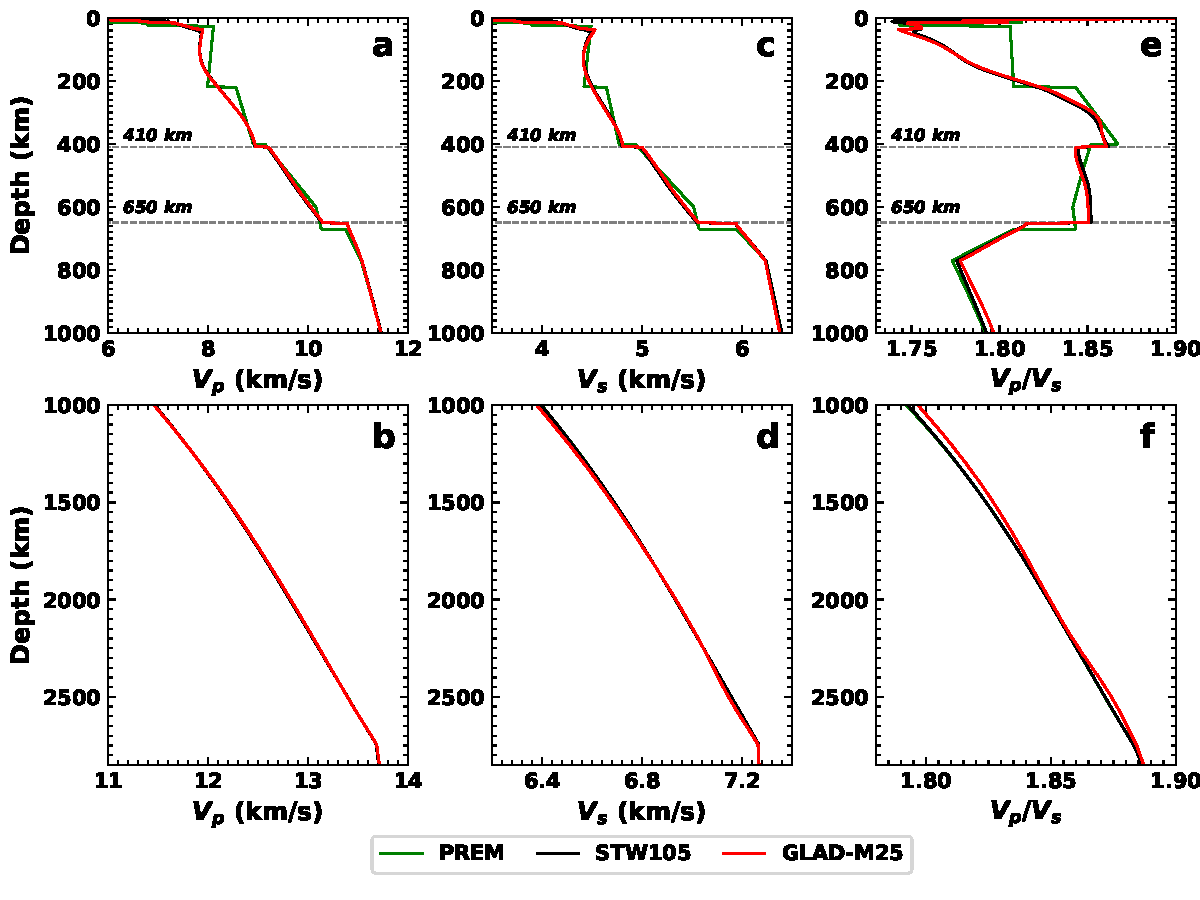
\includegraphics[width=0.8\textwidth]{figures/1d_profile.pdf}
  \caption{\small{1D radial shear and compressional wavespeed profiles for GLAD-M25, STW105, and PREM.
  The reference frequency for physical dispersion is~1~Hz.}}
  \label{fig:global-average}
\end{figure}

\begin{figure}
  \centering
  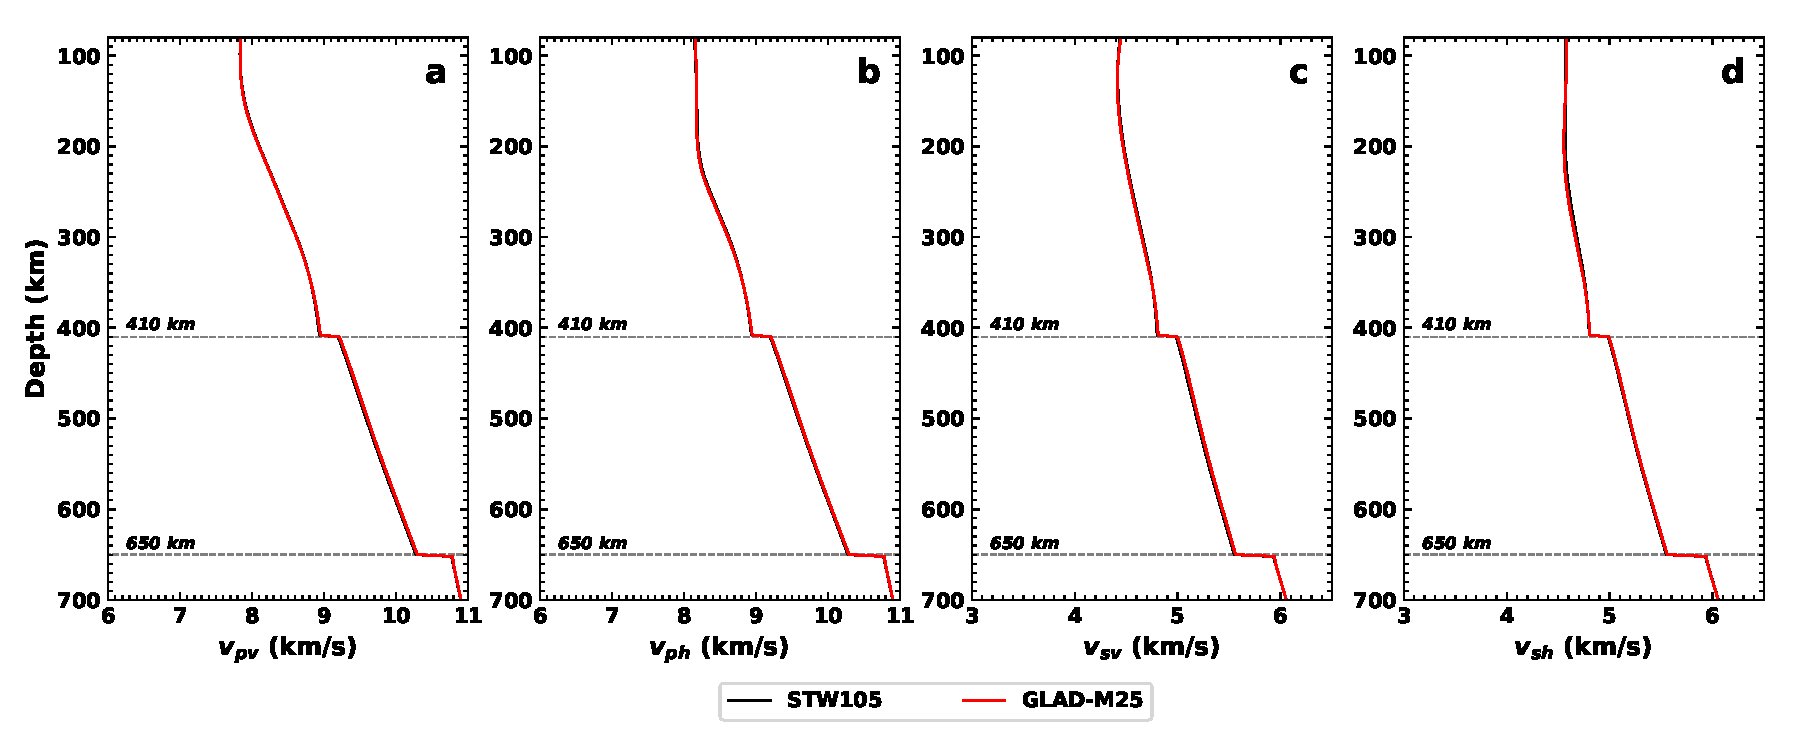
\includegraphics[width=0.9\textwidth]{figures/1d_profile_ra.pdf}
  \caption{\small{1D radial-anisotropic shear and compressional wavespeed profiles for GLAD-M25 and STW105. The reference frequency for physical dispersion is~1~mHz.}}
  \label{fig:global-ra-average}
\end{figure}

\newpage
\section{Spherical harmonic model expansion}
\label{sec:shanalysis}

In this appendix we express model GLAD-M25 in a spherical harmonic basis
to facilitate easy plotting, analysis, and comparisons with other models.
The resulting spherical harmonic model should only be used for these purposes, not for numerical simulations, which should always be based on the fully 3D spectral-element mesh.

To accomplish the transformation,
we first need to transform the 3D mesh --- which includes ellipticity, topography/bathymetry and undulations on internal boundaries --- into a spherical volume.
After these adjustments, we obtain a spectral element mesh for a perfect sphere,
that is, the sort of mesh used for spherically symmetric earth models, such as PREM~\citep{PREM}.

In the spherical mesh, the model may be expressed in the form
\begin{equation}
    m(\mathbf{x})=\sum_{\mathrm{elem}}\sum_{\alpha,\beta,\gamma}m^{\alpha\beta\gamma}\,h_{\alpha}(\xi)\,h_{\beta}(\eta)\,h_{\gamma}(\zeta)\,
    \quad ,
\end{equation}
where~$h_\alpha$ denotes a Lagrange polynomial, and where we have used the invertible mapping
\begin{equation}
    \mathbf{x}=\mathbf{x}(\xi,\eta,\zeta)
    \label{eq:map}
\end{equation}
between spatial points~$\mathbf{x}=\{x,y,z\}$ and Gauss-Lobatto-Legendre (GLL) points in the reference element~$\{\xi,\eta,\zeta\}$~\citep{KoTr99}.

Our goal is to expand our spectral-element model in a spherical harmonic basis, i.e.,
\begin{equation}
    m(\mathbf{x})=\sum_{n=0}^N\sum_{\ell = 0}^L\sum_{m=-\ell}^\ell {}_nC_{\ell m}\,R_n(r)\,Y_{\ell m}(\theta,\phi)
    \quad ,
    \label{eq:m}
\end{equation}
where~$r$ denotes the radius, $\theta$ colatitude, and~$\phi$ longitude.
We choose a radial basis of the form~$R_n(r)$\,, $n=0,\ldots,N$\,,
e.g., layers or B-splines.
These radial basis functions need to be chosen sufficiently dense to mimic the density of the radial spectral element mesh.
The radial basis may or may not be orthogonal,
i.e.,
\begin{equation}
    \int_b^a R_{n'}(r)\,R_{n}(r)\,r^2\mathrm{d}r = A_{n'n}
    \quad ,
    \label{eq:R}
\end{equation}
where~$b$ denotes the radius of the CMB and~$a$ the free surface.
The matrix elements~$A_{n'n}$ define a positive definite matrix which is invertible.
As lateral basis functions we use fully normalized spherical harmonics~$Y_{\ell m}(\theta,\phi)$\,, $\ell=0,\ldots,L$ and $m=\mbox{}-\ell,\ldots,\ell$\,, i.e.,~\citep{DT98}
\begin{equation}
    \int_0^{2\pi}\int_0^\pi Y^*_{\ell'm'}(\theta,\phi)\,Y_{\ell m}(\theta,\phi)\,\sin\theta\,\mathrm{d}\theta\,\mathrm{d}\phi = \delta_{\ell' \ell}\,\delta_{m'm}
    \quad ,
    \label{eq:Y}
\end{equation}
where an asterisk denotes complex conjugation.
The maximum degree~$L$ needs to be chosen to resolve the spectral-element mesh laterally.

To obtain the expansion coefficients~${}_nC_{\ell m}$\,, we multiply Eqn.~(\ref{eq:m}) by
$R_{n'}(r)\,Y^*_{\ell' m'}(\theta,\phi)$ and integrate over the volume of the mantle and crust,~$V$\,, using Eqns.~(\ref{eq:R} and~(\ref{eq:Y}):
\begin{equation}
    \int_V m(\mathbf{x})\,R_{n'}(r)\,Y^*_{\ell' m'}(\theta,\phi)\,\mathrm{d}^3\mathbf{x}=\sum_{n=0}^N {}_nC_{\ell' m'}\,A_{n'n}
    \quad ,
\end{equation}
We evaluate the integral on the left using GLL quadrature~\citep{KoTr99}:
\begin{equation}
    \sum_{\mathrm{elem}}\sum_{\alpha,\beta,\gamma}\omega_\alpha\,\omega_\beta\,\omega_\gamma\,m^{\alpha\beta\gamma}\,J^{\alpha\beta\gamma}\,R_{n'}^{\alpha\beta\gamma}\,Y_{\ell'm'}^{*\,\alpha\beta\gamma}
    =\sum_{n=0}^N {}_nC_{\ell' m'}\,A_{n'n}
    \quad .
\end{equation}
Here~$\omega_\alpha$ denotes a GLL quadrature weight,
$J_{\alpha\beta\gamma}$ the Jacobian of the mapping~(\ref{eq:map}) evaluated on the GLL points,
and $R_{n'}^{\alpha\beta\gamma}$ and $Y_{\ell'm'}^{*\,\alpha\beta\gamma}$ the values of the radial and spherical harmonic basis functions at a GLL point.

Finally, the desired model coefficients may be obtained ---one combination of $n$\,, $\ell$\,, and $m$ at a time--- via
\begin{equation}
    {}_nC_{\ell m}=\sum_{n'}A^{-1}_{nn'}\sum_{\mathrm{elem}}\sum_{\alpha,\beta,\gamma}\omega_\alpha\,\omega_\beta\,\omega_\gamma\,m^{\alpha\beta\gamma}\,J^{\alpha\beta\gamma}\,R_{n'}^{\alpha\beta\gamma}\,Y_{\ell m}^{*\,\alpha\beta\gamma}
    \quad ,
    \label{eq:Cnlm}
\end{equation}
where~$A^{-1}$ denotes the inverse of the~$N\times N$ matrix~$A$.
Expressions of the form~(\ref{eq:Cnlm}) are commonplace in spectral-element simulations,
and thus easily calculated.

The normalized power per degree~$\ell$ may be calculated via
\begin{equation}
    \sigma_\ell^2=\frac{1}{2\ell+1}\,
    \sum_{n' = 0}^N\sum_{n = 0}^N\sum_{m = -\ell}^\ell\,A_{n'n}\,{}_{n'}C^*_{\ell m}\,{}_{n}C_{\ell m}
    \quad .
\end{equation}
Alternatively,
one may wish to calculate the power per degree as a function of radius,
which is determined via
\begin{equation}
    \Sigma_\ell^2(r)=\frac{1}{2\ell+1}\,
    \sum_{n' = 0}^N\sum_{n = 0}^N\sum_{m = -\ell}^\ell\,R_{n'}(r)\,R_{n}(r)\,{}_{n'}C^*_{\ell m}\,{}_{n}C_{\ell m}
    \quad .
\end{equation}

Instead of the complex spherical harmonic model expansion~(\ref{eq:m}),
we may wish to use a real spherical harmonic expansion of the form~\citep[][Section~B.8, Eqn.~B.99]{DT98}
\begin{equation}
\begin{split}
    m(\mathbf{x}) \ = & \ \sum_{n=0}^N\sum_{\ell = 0}^L \left[ {}_na_{\ell 0}\,R_n(r)\,X_{\ell 0}(\theta)
   +\sqrt{2}\sum_{m=1}^\ell R_n(r)\,({}_na_{\ell m}\,\cos m\phi+{}_nb_{\ell m}\,\sin m\phi)\,X_{\ell m}(\theta)\right]
    \quad ,
\end{split}
    \label{eq:mreal}
\end{equation}
where~\citep[][Eqn.~B.30]{DT98}
\begin{equation}
    Y_{\ell m}(\theta,\phi)=X_{\ell m}(\theta)\exp(i m\phi)
    \quad ,
\end{equation}
and where
\begin{equation}
    {}_na_{\ell 0}=\sum_{n'}A^{-1}_{nn'}\sum_{\mathrm{elem}}\sum_{\alpha,\beta,\gamma}\omega_\alpha\,\omega_\beta\,\omega_\gamma\,m^{\alpha\beta\gamma}\,J^{\alpha\beta\gamma}\,R_{n'}^{\alpha\beta\gamma}\,X_{\ell m}^{\alpha\beta\gamma}
    \quad ,
\end{equation}
and for~$1\le m\le \ell$
\begin{equation}
    {}_na_{\ell m}=\sqrt{2}\,\sum_{n'}A^{-1}_{nn'}\sum_{\mathrm{elem}}\sum_{\alpha,\beta,\gamma}\omega_\alpha\,\omega_\beta\,\omega_\gamma\,m^{\alpha\beta\gamma}\,J^{\alpha\beta\gamma}\,R_{n'}^{\alpha\beta\gamma}\,X_{\ell m}^{\alpha\beta\gamma}\,(\cos m \phi)^{\alpha\beta\gamma}
    \quad ,
\end{equation}
\begin{equation}
    {}_nb_{\ell m}=\sqrt{2}\,\sum_{n'}A^{-1}_{nn'}\sum_{\mathrm{elem}}\sum_{\alpha,\beta,\gamma}\omega_\alpha\,\omega_\beta\,\omega_\gamma\,m^{\alpha\beta\gamma}\,J^{\alpha\beta\gamma}\,R_{n'}^{\alpha\beta\gamma}\,X_{\ell m}^{\alpha\beta\gamma}\,(\sin m \phi)^{\alpha\beta\gamma}
    \quad .
\end{equation}
The normalized power per degree~$\ell$ may then be calculated via
\begin{equation}
    \sigma_\ell^2=\frac{1}{2\ell+1}\,\sum_{n'=0}^N\,\sum_{n=0}^N\,A_{n'n}\,\left[{}_{n'}a_{\ell 0}\,{}_{n}a_{\ell 0}+\sum_{m=1}^\ell({}_{n'}a_{\ell m}\,{}_na_{\ell m}+{}_{n'}b_{\ell m}\,{}_nb_{\ell m})\right]
    \quad ,
    \label{eq:powerdegree}
\end{equation}
and the normalized power per degree as a function of radius is determined via
\begin{equation}
    \Sigma_\ell^2(r)=\frac{1}{2\ell+1}\,\sum_{n'=0}^N\,\sum_{n=0}^N\,R_{n'}(r)\,R_{n}(r)\,\left[{}_{n'}a_{\ell 0}\,{}_{n}a_{\ell 0}+\sum_{m=1}^\ell({}_{n'}a_{\ell m}\,{}_na_{\ell m}+{}_{n'}b_{\ell m}\,{}_nb_{\ell m})\right]
    \quad .
    \label{eq:powerdegreeradius}
\end{equation}
In Fig.~\ref{fig:powerspectra} we plot the normalized power per degree~$\ell$ for models S362ANI, GLAD-M15, and GLAD-M25,
and Fig.~\ref{fig:powerspectraradius} shows the normalized power per degree as a function of radius
for the same set of models.

\begin{figure}
  \centering
  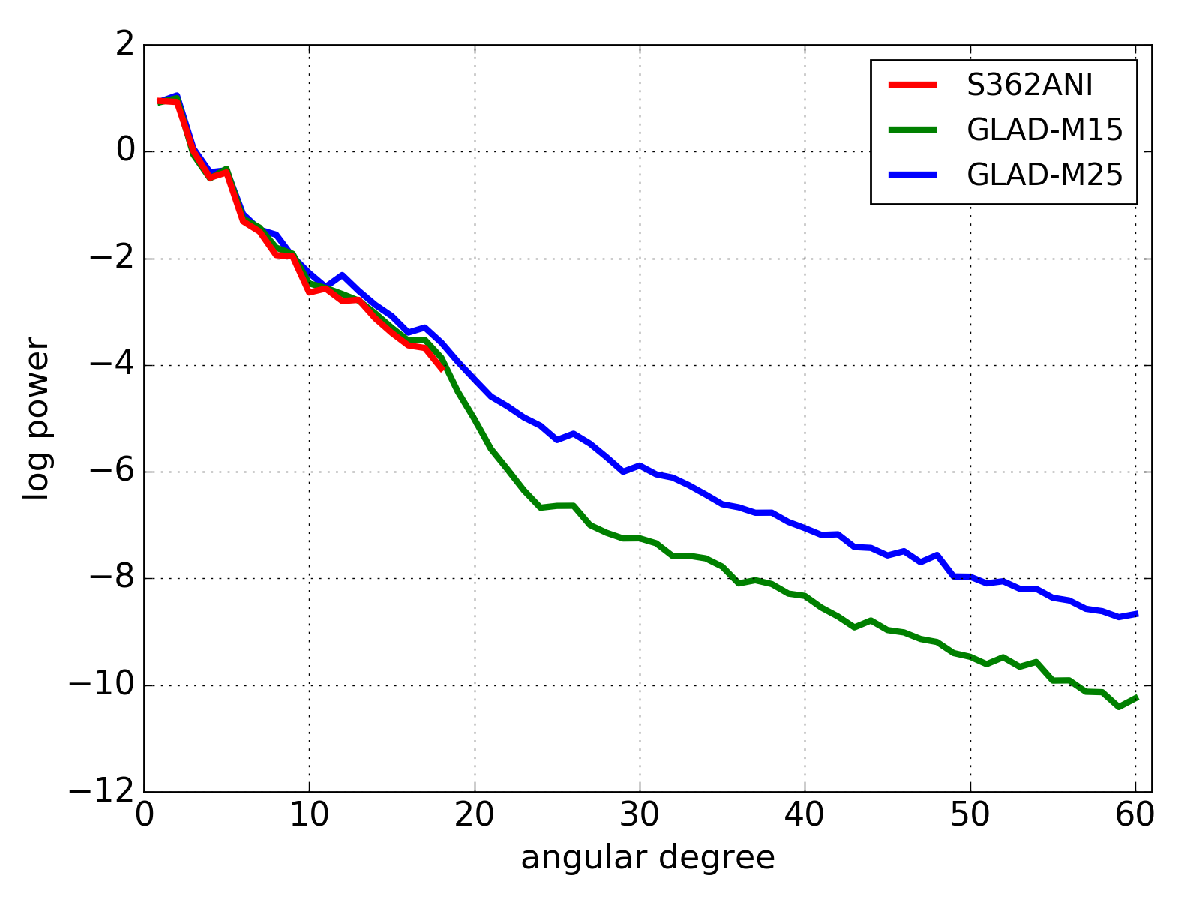
\includegraphics[width=0.5\textwidth]{figures/power.pdf}
  \caption{\small{Normalized power per degree~$\ell$, based on Eqn.~(\ref{eq:powerdegree}), for models S362ANI (red), GLAD-M15 (green), and GLAD-M25 (blue).
  The calculation includes depths greater than 120~km.
  Model S362ANI has no power beyond degree~18,
  and model S40RTS has no power beyond degree~40.
  (Courtesy of Caio Ciardelli.)
  }}
  \label{fig:powerspectra}
\end{figure}
% In Fig.~\ref{fig:powerspectra} we plot the normalized power per degree~$\ell$ for models S362ANI, S40RTS, GLAD-M15, and GLAD-M25,
% and Fig.~\ref{fig:powerspectraradius} shows the normalized power per degree as a function of radius
% for the same set of models.

% \begin{figure}
%   \centering
%   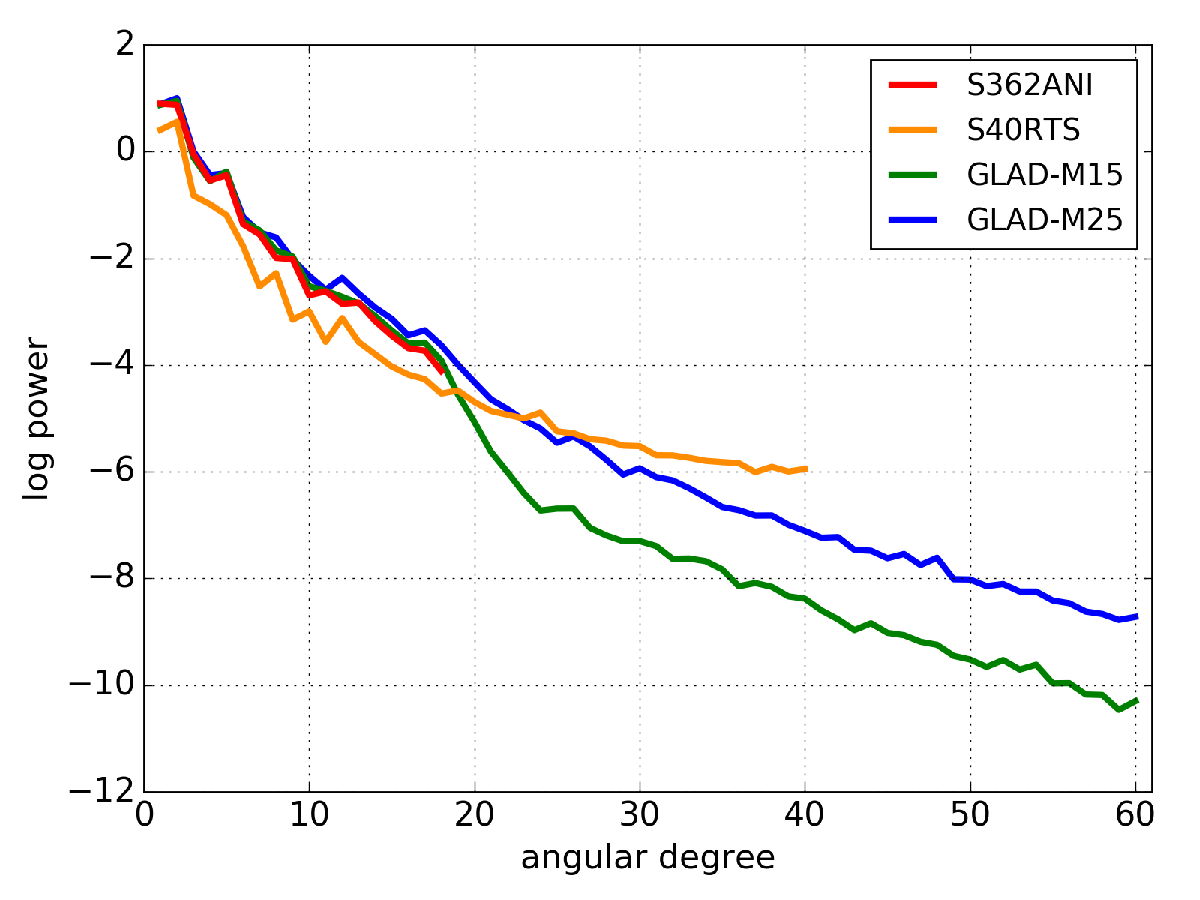
\includegraphics[width=0.5\textwidth]{figures/power2.pdf}
%   \caption{\small{Normalized power per degree~$\ell$, based on Eqn.~(\ref{eq:powerdegree}), for models S362ANI (red), S40RTS (orange), GLAD-M15 (green), and GLAD-M25 (blue).
%   The calculation includes depths greater than 120~km.
%   Model S362ANI has no power beyond degree~18,
%   and model S40RTS has no power beyond degree~40.
%   (Courtesy of Caio Ciardelli.)
%   }}
%   \label{fig:powerspectra}
% \end{figure}

\end{document}
